%!TEX root = ../template.tex
%%%%%%%%%%%%%%%%%%%%%%%%%%%%%%%%%%%%%%%%%%%%%%%%%%%%%%%%%%%%%%%%%%%%
%% chapter3_HardwareDesign.tex
%% NOVA thesis document file
%%
%% Chapter with the Hardware Design part
%%%%%%%%%%%%%%%%%%%%%%%%%%%%%%%%%%%%%%%%%%%%%%%%%%%%%%%%%%%%%%%%%%%%

\typeout{NT FILE chapter3_HardwareDesign.tex}

\chapter{Hardware Design}\label{cha:chapter3_HardwareDesign}

Meter aqui um pequena introdução do que e mostrado neste capitulo e descrição de seccoes

%SSSSSSSSSSSSSSSSSSSSSSSSSSSSSSSSSSSSSSSSSSSSSSSSSSSSSSSSSSSSSSSSSSSSSSSSSSSS
\section{Architecture and Component Selection}\label{sec:31_Architecture}

The system's desired specifications and requirements exposed throughout Section~\ref{sec:II_Specs} allow a redesign of its current architecture (Figure~\ref{fig:architecture_original}), which is presented in Figure~\ref{fig:architecture_new}.

% meter aqui o NOVO diagrama de blocos -- INACABADO;
\begin{figure}[h]
	\centering
	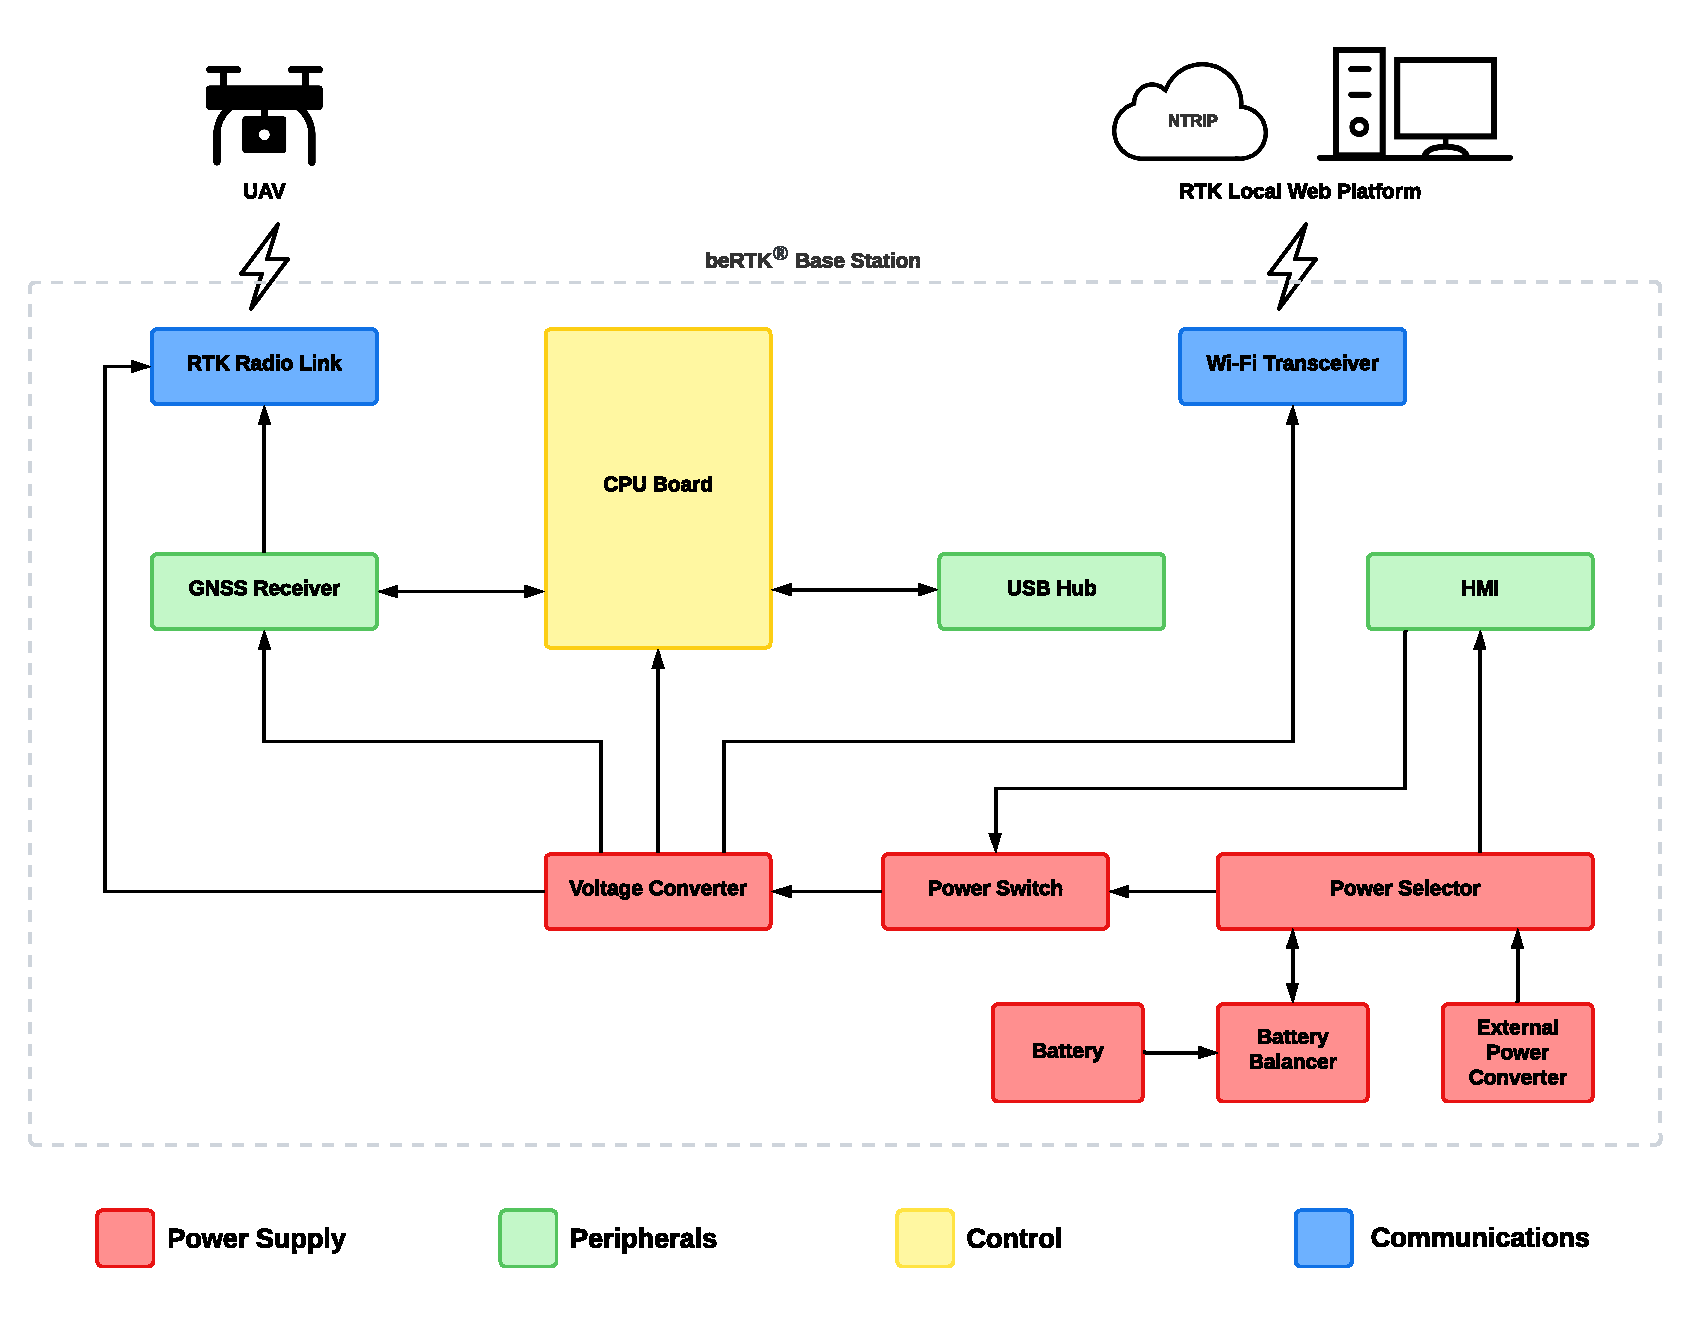
\includegraphics[width=1.0\textwidth]{Chapters/Figures/new_architecture_2.pdf}
	\caption{beRTK\textsuperscript{\textregistered} Base Station's redesigned block diagram.}
	\label{fig:architecture_new}
\end{figure}

%VER SE ESTA ORDEM DE SUBCAPITULOS É BOA O SUFICIENTE, ou se tenho de a alterar

%sSsSsSsSsSsSsSsSsSsSsSsSsSsSsSsSsSsSsSsSsSsSsSsSsSsSsSsSsSsSsSsSsSsSsSsSsSsS
\subsection{Control}\label{sec:311_Control}

Starting from the control subgroup, the only component to be selected was a single-board computer able to replace the previously used Raspberry Pi 4 Model B; this means the chosen device would have to be able to carry out a pre-determined set of instructions crucial for the operation of the base station. Such requirement is presented in Section~\ref{sec:II_FCT_requirements} -- requirement \textbf{RTKBS.MAIN.FCT.030}, which proposes the use of a single-board computer (SBC).
The set of instructions performed by the original beRTK\textsuperscript{\textregistered} base station is carried out by a Raspberry Pi 4 Model B computer (described in Section~\ref{sec:II_architecture_Control}), therefore, an element with a comparable computational power as this computer would be ideal. The Raspberry Pi Foundation offers a variety of solutions for many project ideas\footnote[7]{The Raspberry Pi Foundation's hardware offers are available at \url{https://www.raspberrypi.com/products/}.}, and since the operations intended for the beRTK\textsuperscript{\textregistered} base station are so well performed by the Raspberry Pi 4 Model B, it would be worth looking through the array of Raspberry Pi products in order to find a good solution. Research leads to the Raspberry Pi Compute Module 4.
This compact module not only has a small form factor when compared with the Raspberry Pi 4 Model B, but it also bears its computational power, thanks to the same processor (a Broadcom BCM2711 quad-core Cortex-A72 (ARM v8) 64-bit SoC @ 1.5GHz). This makes it a great option for the system's control unit~\cite{CM4}.

%meter imagem CM4:
\begin{figure}[h]
	\centering
	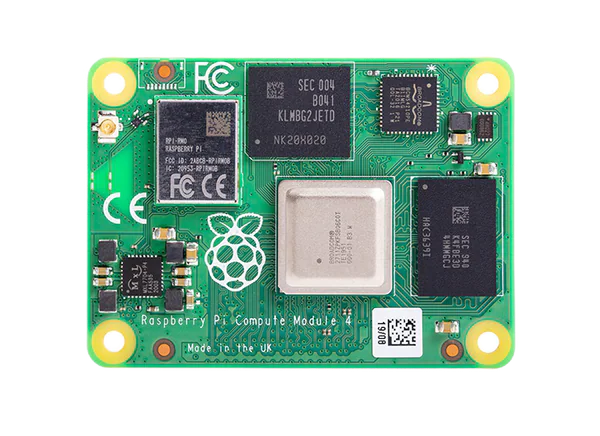
\includegraphics[width=0.5\textwidth]{Chapters/Figures/CM4.png}
	\caption{The Raspberry Pi Compute Module 4 (CM4)~\cite{CM4}.}
	\label{fig:CM4}
\end{figure}

One can choose from thirty-two CM4 variants which differ from each other on RAM and eMMC flash, as well as with or without wireless capabilities.

%sSsSsSsSsSsSsSsSsSsSsSsSsSsSsSsSsSsSsSsSsSsSsSsSsSsSsSsSsSsSsSsSsSsSsSsSsSsS
\subsection{Peripherals and Communications}\label{sec:312_Peripherals_Communications}

Since this module is intended to be an embedded solution without any of the external ports present in the Raspberry Pi 4 Model B, the relevant ones must be included in the proposed solution, which in this case are USB and HDMI. The CM4 provides all the necessary pins for the implementation of two HDMI connectors on its carrier board (in this case the base station); however, when it comes to using its USB interface, the user must add a USB hub, since only two USB data pins are provided, along with a USB On-The-Go (OTG) pin. The latter, is used in order to define the CM4 as either a host or a slave~\cite{CM4}.

%meter imagem do HUB usb: LAN9514

In order to enable such data transfers, the base station would need a component designed to allow the setup of both upstream and downstream USB ports. The Raspberry Pi 3 Model B uses a chip known as LAN9514, which is a four-port USB hub with Ethernet functionality. Since this chip has the needed characteristics for the setup of the CM4's USB interface, it was chosen as the main module concerning USB data transfer.

The datasheet for LAN9514 details the chip as a 10/100 Ethernet controller, as well as a USB 2.0 hub with four downstream ports and one upstream port, and targets it for desktop computers and embedded systems, among other uses~\cite{LAN9514}. The LAN9514 also fits the Peripherals subgroup, along with the ZED-F9P GNSS receiver and the HMI, the latter of which bridges the user-device gap via a simple on/off button, LED indicators for both battery status and power source indication and a single connector intended for an external power source, satisfying requirement \textbf{RTKBS.MAIN.PWS.050}, as well as all the requirements defined in Section~\ref{sec:II_HMI_requirements}.

It is also worth mentioning that, referring to requirements \textbf{RTKBS.MAIN.FCT.020} and \textbf{RTKBS.MAIN.FCT.040}, which correspond to the GNSS receiver (ZED-F9P) and the Wi-Fi transceiver (Digi XBee\textsuperscript{\textregistered} 3), respectively, there were no changes in such elements for the new beRTK\textsuperscript{\textregistered}'s proposed solution.

%sSsSsSsSsSsSsSsSsSsSsSsSsSsSsSsSsSsSsSsSsSsSsSsSsSsSsSsSsSsSsSsSsSsSsSsSsSsS
\subsection{Power Supply}\label{sec:313_PowerSupply}

The secondary power arrangement in the original beRTK\textsuperscript{\textregistered} design features two external batteries that would feed the entire system once the mains power supply was disconnected. This form of supply poses considerable disadvantages when it comes to a continuous operation, due to the impractical need of removing the batteries in order to charge them. In the system's power supply subgroup, this was the main improvement to be made following the requirements defined in Section~\ref{sec:II_PWS_requirements}. For that, the base station's enclosure sould count on an internal battery (requirement \textbf{RTKBS.MAIN.PWS.020}) that must not be removed (such battery could be comprised of either a single or multi-cell arrangement) on which the system could rely once the external power supply was disconnected. This idea would help meet requirement \textbf{RTKBS.MAIN.MEC.030}, proposing however a new issue, namely, the charging of the internal battery arrangement.
%meter hyperLINK PARA CADA REQUIREMENT

The original beRTK\textsuperscript{\textregistered}'s design also features a prioritized PowerPath\textsuperscript{\texttrademark} controller, as mentioned in Section~\ref{sec:II_architecture_PowerSupply}.
As per Analog Devices, a PowerPath\textsuperscript{\texttrademark} controller is a device able to control the flow of power through a system, while also selecting its power source.
With this in mind, a wise starting point for the research of a power selector able to provide a smooth transition between an external and internal supply would be from Analog Devices' power management ICs; specifically, from the battery charger IC catalogue. The most well-suited IC found was LTC4012, which is a high efficiency, multi-chemistry battery charger with PowerPath\textsuperscript{\texttrademark} control. This battery charger offers an adjustable output voltage, as well as the option to program a charging current for the circuit's internal battery~\cite{LTC4012}.

Taking into account requirement \textbf{RTKBS.MAIN.PWS.010} -- which regards the system's input \gls{DC} voltage (from +7VDC to +22VDC) -- and the battery charger's input voltage range (from +6VDC to +28VDC), the intermediary value of +15VDC was chosen as the main DC input voltage for the system -- supplied by an external power adapter. It must be noted that the calculations made throughout the circuit design phase take into consideration an external supply voltage that can range from +15VDC to +22VDC.
%falar de como a PWM permite um switching smooth entre external power para as baterias - meter requirement(s) que condigam com isto

%depois falar do sistema operativo - meter requirement(s) que condigam com isto

%depois falar da local web platform - meter requirement(s) que condigam com isto
	% da configuraçao dos parametros da base atraves dessa plataforma
	% dos log que podem ser obtidos atraves da operaçao da base
	%- meter requirement(s) que condigam com tudo

%SSSSSSSSSSSSSSSSSSSSSSSSSSSSSSSSSSSSSSSSSSSSSSSSSSSSSSSSSSSSSSSSSSSSSSSSSSSS
\section{Circuit Design}\label{sec:32_Circuit}

%meter uma pequena introduçao a dizer que usei o kicad e que segui uma metodologia qualquer

%sSsSsSsSsSsSsSsSsSsSsSsSsSsSsSsSsSsSsSsSsSsSsSsSsSsSsSsSsSsSsSsSsSsSsSsSsSsS
\subsection{Power Supply}\label{sec:321_POWERSUPPLY}
	%mini introdução

%s--Ss--Ss--Ss--Ss--Ss--Ss--Ss--Ss--Ss--Ss--Ss--Ss--Ss--Ss--Ss--Ss--Ss--Ss--S
\subsubsection{Power Selector}\label{sec:3211_LTC4012}

\paragraph{Programming the Charge Current}	When it comes to powering the system through different sources, maintaining its continuous operation when switching between said sources is crucial. The LTC4012 battery charger is able to accomplish just that: this buck converter relies on a synchronous quasi-constant frequency \gls{PWM} control architecture and is able to provide a connected battery pack with a charge current programmed through external resistors. Since it does not have a built-in termination, it is capable of charging a broad range of batteries at a maximized rate and effieciency -- for a given established power level --, due to an existing \gls{AC} adapter current limiting feature, possible to program and monitor via an external sense resistor. For this project, an arrangement of two rechargeable Lithium-ion (Li-ion) cells in series (also known as a ``2S Li-ion battery'') was chosen as the backup battery pack for the system, with each of the cells offering $3,350$mAh worth of capacity. It must be noted that a set of two cells in series does not alter the pack's total capacity, therefore this same specification will remain the same for the backup battery -- $3,350$mAh.

With this in mind, studying the battery cell's datasheet reveals that each battery -- and therefore, the 2S arrangement -- is capable of being charged with a recommended standard charge of $1,700$mA~\cite{INR18650-35E}.
Figure~\ref{fig:battery2S} and Table~\ref{tab:battery2S} show a close-up representation and typical characteristics of a single cell, respectively.

%imagem e Table da bateria aqui:
\begin{figure}[h]
	\centering
	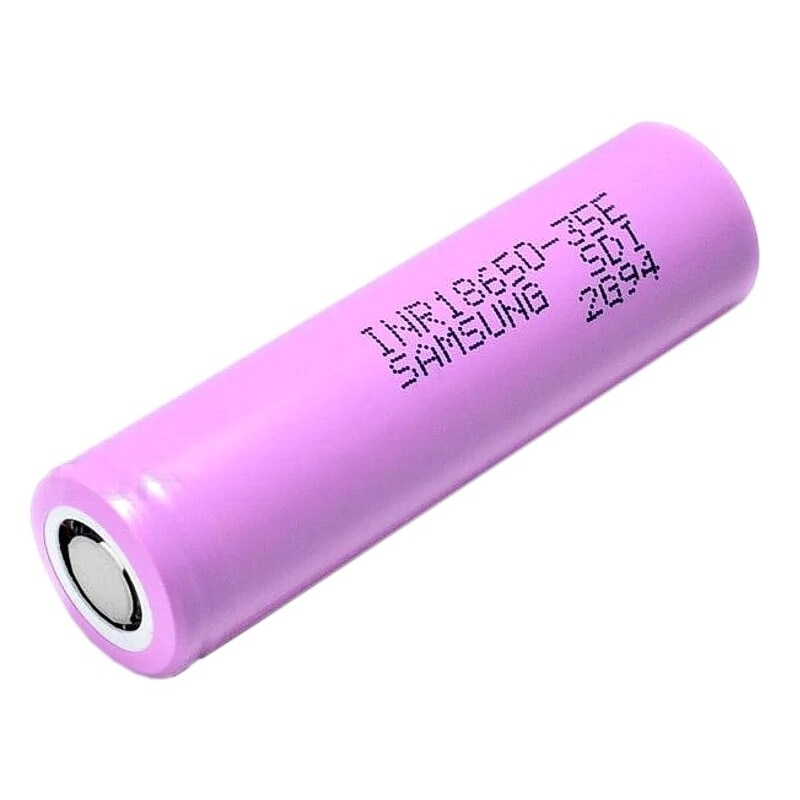
\includegraphics[width=0.4\textwidth]{Chapters/Figures/chapter3/bateria-li-ion-mr-18650-3-6v-3500mah-samsung-inr18650-35e.jpg}
	\caption{Visual representation of the type of battery cell used.}
	\label{fig:battery2S}
\end{figure}

\begingroup
\begin{table}[h]
	\caption{Typical characteristics of the type of battery cell used~\cite{INR18650-35E}.}
	\label{tab:battery2S}
	\centering%@{}l@{}@{}c@{}@{}c@{}@{}c@{}@{}c@{}
    % \setlength{\tabcolsep}{10pt} % Default value: 6pt
    % \renewcommand{\arraystretch}{1.5} % Default value: 1
	\begin{tabular}{lc}
        \toprule
        \textbf{Specification} & \textbf{Value} \\
        \midrule
        Manufacturer & Samsung SDI \\
        \midrule
        Model & INR18650-35E \\
        \midrule
		Size & 18650 \\
		\midrule
		Chemistry & Li-ion \\
		\midrule
		Capacity & 3,350mAh \\
        \midrule
		Charging Cycle Termination Voltage & 4.20V $\pm$ 0.05V \\
		\midrule
		Nominal Voltage & 3.60V \\
        \midrule
		Charging Current (standard charge) & 1,700mA\\
		\midrule
		Charging Current (for life cycle) & 1,020mA\\
		\midrule
		Maximum Charge Current (not for life cycle) & 2,000mA \\
		\midrule
		Minimum Charge Current & 68mA \\
		\midrule
		Maximum Discharge Current (continuous discharge) & 8,000mA \\
		\midrule
		Maximum Discharge Current (not for continuous discharge) & 13,000mA \\
		\midrule
		Discharge Cut-off Voltage & 2.65V \\
        \bottomrule
    \end{tabular}
\end{table}
\endgroup

Table~\ref{tab:battery2S} specifies that each battery provides a charging cycle termination voltage of approximately 4.20V, which bespeaks that the 2S arrangement adds up to a total of (approximately) 8.4V of backup energy.

It is possible to calculate an estimate of the system's battery life using expression~(\ref{eq:battery_life}):

\begin{equation}\label{eq:battery_life}
    \textrm{Battery Life} = \frac{\textrm{Battery Capacity (mAh)}}{\textrm{Load Current (mAh)}} = \frac{3350}{1000} = 3.35 \textrm{ hours}\,\medskip
\end{equation}

\noindent Assuming a total system load current of approximately $1,000$mA results in an expected total battery life of roughly 3.35 hours. That estimate corresponds to, roughly, three-and-a-half hours of work time. Of course one must account for the unideal characteristics of the real world acting upon the system, but nevertheless, this expression serves as a guideline/reminder for an expected power consumption of the base station's circuit. 

The LTC4012 datasheet provides a helpful typical application circuit, as well as the device's application information. These two key sections of the document allowed an adapted development of the power selection circuit of the new beRTK\textsuperscript{\textregistered}, presented by the schematic diagram in Figure~\ref{fig:LTC4012_circuit}. Following the application information of the product started by programming the charge current which would be used to replenish the energy back to the battery pack. For that, formula~\ref{eq:i_chrg} is provided:

\begin{equation}\label{eq:i_chrg}
    I_{CHRG}=\frac{R_{IN}}{R_{SENSE}} \cdot \left(\frac{1.2085\textrm{V}}{R_{PROG}}-11.67\mu\textrm{A}\right)\,\medskip
\end{equation}

\noindent The $I_{CHRG}$ charge current is programmed by selecting the $R_{IN}$, $R_{SENSE}$ and $R_{PROG}$ resistors. $R_{SENSE}$ (sense resistor) can be selected through expression~(\ref{eq:r_sense}),

\begin{equation}\label{eq:r_sense}
    R_{SENSE}=\frac{100 \textrm{mV}}{I_{MAX}}\,,\medskip
\end{equation}
where $I_{MAX}$ corresponds to the maximum $I_{CHRG}$ charge current desired for the charging process. As per Table~\ref{tab:battery2S}, the battery pack allows a maximum charge current of $2,000$mA, but this value does not account for the maintenance of each cell's health. For that, a standard charging current of $1,700$mA is mentioned in the datasheet; in C-rate units, this charging current rate corresponds to 0.5C, since the explicit 1C rate for this type of cell is equal to $3,400$mA\footnote[8]{In the C-rate standard, 1C corresponds to a charging from 0 to 100\% in the span of one hour. The higher the C-rate coefficient, the faster the charge, and vice-versa. For example, a rate of 2C corresponds to thirty minutes of charge time and 0.5C to two hours.}~\cite{C-rate}.
However, it is also pointed out that, in order to maintain the batteries' health as pristine as possible (thus prolonging their life cycle), a charge current of $1,020$mA -- i.e. maintaining the cell's C-rate of 0.3C -- would have to be employed. Choosing a maximum charge current of $I_{MAX}=1,020$mA results in an $R_{SENSE}$ value of 0.098$\Omega$ (98m$\Omega$), according to~(\ref{eq:r_sense}) (represented in the schematic of Figure~\ref{fig:LTC4012_circuit} by R12). Therefore, the value of $I_{MAX}=1,020$mA is hereby defined as the 1C rate of the new beRTK\textsuperscript{\textregistered}'s battery pack. It should also be noted that the target sense voltage of 100mV can differ in order to accomodate standard $R_{SENSE}$ values available on the market, however lower values are likely to cause inaccuracies when it comes to current regulation.

% meter aqui circuito do LTC4012:
\begin{figure}[h]
	\centering
	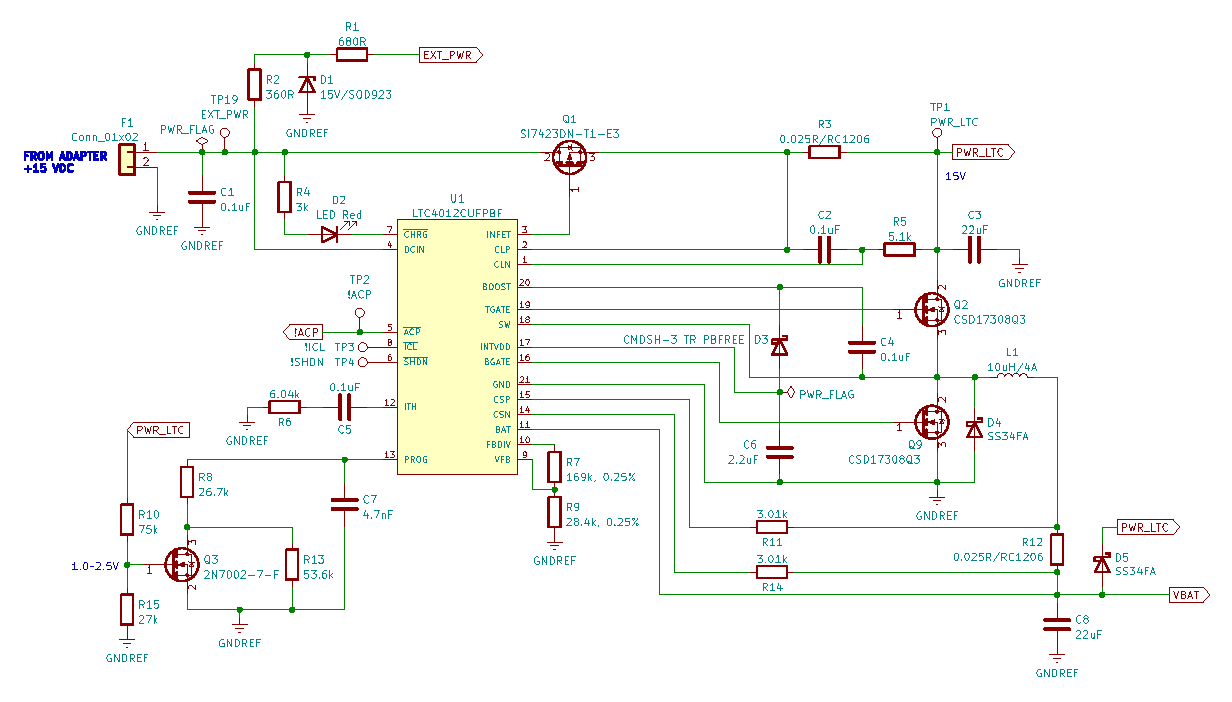
\includegraphics[width=1.0\textwidth]{Chapters/Figures/chapter3/Power_Supply_and_Selection.pdf}
	\caption{beRTK\textsuperscript{\textregistered} Base Station's Power Supply and Selection schematic diagram.}
	\label{fig:LTC4012_circuit}
\end{figure}

It is established in the documentation that the LTC4012 provides the best performance with two equal 3.01k$\Omega$ $R_{IN}$ input resistors\footnote[9]{Other input resistor values can also be used in order to adjust to different standard sense resistor value that could be chosen~\cite{LTC4012}.} (represented in Figure~\ref{fig:LTC4012_circuit} by R11 and R14). This input resistor value is used for the calculation of the minimum resistance required between the PROG pin and \gls{GND}, given by (\ref{eq:r_prog}).

\begin{equation}\label{eq:r_prog}
    R_{PROG (MIN)}=\frac{1.2085 \textrm{V} \cdot R_{IN}}{0.1 \textrm{V} + 11.67 \mu \textrm{A} \cdot R_{IN}} \approx 26.9 \textrm{k}\Omega \,\medskip
\end{equation}

\noindent Expression (\ref{eq:r_prog}) results in a minimum $R_{PROG}$ value of approximately 26.9k$\Omega$, and connecting a resistor of this value between the PROG pin and GND is enough to control the maximum charge current of $I_{MAX}$ (i.e. 1C).

% \noindent Expression (\ref{eq:r_prog}) results in a minimum $R_{PROG}$ value of approximately 26.9k$\Omega$, and connecting a resistor of this value between the PROG pin and GND would be sufficient if the only charge current rate defined was $I_{MAX}$ (i.e. 1C).
% However, when batteries discharge to a voltage level below their minimum specified recommendation (in the case of the cells used, 2.5V), they suffer internal damage, which results -- in the long run -- in a loss of battery life.
% Therefore, when the aforesaid situation occurs, the charging process should be done with a low initial charge current. Such practice also ensures an overall safe charging of the baterries, regardless of whether or not a heavy discharge has taken palce.
% The LTC4012 charger allows a specific charging control process for the battery pack by altering the resistance between the PROG pin and GND, designated as a ``two-level'' charge. This charging process is achieved via the switching of a control transistor (Q3 in Figure~\ref{fig:LTC4012_circuit}) which, when turned off, cuts down the charge current to $\frac{I_{MAX}}{10}$ (i.e. C/10), only allowing the full $I_{MAX}$ current for a ``bulk charge'' when turned on. In the schematic of Figure~\ref{fig:LTC4012_circuit}, the two-level approach is implemented through transistor Q3, resistors R8 and R13 and capacitor C7. Connecting the gate of Q3 to the battery supply rail ($\mathrm{V_{BAT}}$ net in Figure~\ref{fig:LTC4012_circuit}) serves the purpose of allowing transistor Q3 to exit or enter its active zone, in order to subsequently grant both levels of charge current available with the implemented method. When the battery pack's voltage dips to a value equal to or below 2.5V -- i.e. when it reaches a heavy discharge status --, Q3 is switched on, increasing (MENTIRA! ELE DIMINUI A RESISTENCIA...) the resistance between PROG and GND. For that, the recommended transistor to use (from the LTC4012 datasheet) is the 2N7002 N-channel \gls{FET}~\cite{2N7002}. This FET holds a gate threshold voltage between 1.0V and 2.5V.
%DESCARTEI O 2-LEVEL CHARGE.

With the calculated values for resistors $R_{IN}$, $R_{SENSE}$ and $R_{PROG}$ it is then possible to obtain a value of $I_{CHRG} = 1,020$mA for the programmed charge current, through expression~(\ref{eq:i_chrg})~\cite{LTC4012}.

\paragraph{Programming the LTC4012 Output Voltage}	An external resistor divider circuit can be assembled in order to set an output voltage for the charger. This circuit is composed by resistors R7 and R9 from Figure~\ref{fig:LTC4012_circuit}, whose approximate values are suggested in the LTC4012 datasheet. For a $V_{BAT}$ voltage of 8.4V, these values are 169k$\Omega$ and 28.4k$\Omega$, respectively, and can be confirmed through equations (\ref{eq:v_bat}) and (\ref{eq:r7_r9}):

\begin{equation}\label{eq:v_bat}
    V_{BAT}=\frac{1.2085\textrm{V} \cdot \left(R7 + R9\right)}{R9}\,\medskip
\end{equation}

\begin{equation}\label{eq:r7_r9}
    R7=R9 \cdot \left(\frac{V_{BAT}}{1.2085\textrm{V}} - 1\right)\,\medskip
\end{equation}

If the selected value of R9 is less than 50k$\Omega$ and the joint value of R7 and R9 surpasses (or at least equals) 200k$\Omega$, then the lowest possible error at the $V_{FB}$ sense input is acheived\footnote[10]{The use of resistors with a tolerance level of 0.25\% is advised to achieve the desired level of accuracy~\cite{LTC4012}.}. It should be noted that the influence of this battery voltage feedback input is present in equations (\ref{eq:v_bat}) and (\ref{eq:r7_r9}), as well as in equations (\ref{eq:i_chrg}) and (\ref{eq:r_prog}), in the form of the nominal 1.2085 pin voltage~\cite{LTC4012}.

\paragraph{Programming the Input Current Limit}	The previous version of the beRTK\textsuperscript{\textregistered} base station presented a power consumption of approximately 3 to 3.5Wh, and one of the requirements of this project is to cut the power consumption down to a maximum of 400mA at +5VDC -- as stated in requirement \textbf{RTKBS.MAIN.PWS.040}. Therefore, a 1.00A external adapter current rating can safely be considered, however, it is best to consider the double of that value, to safely consider high peak currents and discharge problems that may arise.
The LTC4012 datasheet provides a table with common values for a sense resistor dedicated to the programming of the input current limiting -- R3 in Figure~\ref{fig:LTC4012_circuit}. For this case, considering an adapter rating of 2.00A, R3's estimated value would be equal to 0.050$\Omega$ (50m$\Omega$). The value of this sense resistor can also be determined through expression (\ref{eq:r_cl}),

\begin{equation}\label{eq:r_cl}
    R3=\frac{100\textrm{mV}}{I_{LIM}}\,,\medskip
\end{equation}
where $I_{LIM}$ corresponds to the desired maximum current able to be drawn from the external adapter input -- in this case, that value was chosen to be 2.00A. The LTC4012 also provides a pin named $\overline{\mbox{ICL}}$, an active-low indicator output that immediately pulls to GND upon the detection of a reduction of the charge current (due to the aforementioned AC adapter input current limiting).

The switching noise generated by the PWM control architecture and different system components can be canceled out by a low-pass filter consisting of resistor R5 (5.1k$\Omega$) and capacitor C2 (0.1$\mu$F) -- also present in Figure~\ref{fig:LTC4012_circuit} --, between the charger's CLP and CLN pins~\cite{LTC4012}.

% \paragraph{The $\mathbf{\frac{C}{10}}$ $\mathbf{\overline{CHRG}}$ Indicator}	As stated before, when the N-channel FET Q3 (2N7002) is turned off, the maximum charge current allowed is $\frac{I_{MAX}}{10}$, which helps preserve the battery's health. This FET allows the setting of two different values for the total external resistance between the PROG pin and GND of the LTC4012 -- composed by resistors R8 and R13 of Figure~\ref{fig:LTC4012_circuit} --, which enables the programming of the battery pack's charge current. Along with this resistance, the R12 current sense resistor and PWM input resistors (R7 and R9) also play an important role on setting said charge current, since information about the current battery level is necessary so that the device can detect if a heavy discharge has taken place (i.e. the discharge cut-off voltage of 2.65V has been reached), in order to only allow the $\frac{I_{MAX}}{10}$ charge current. The LTC4012 provides a dedicated pin ~\cite{LTC4012}

\paragraph{Input and Output Capacitors}	Within a single system, different circuits can share the same nets, the most common of which are usually power and ground. Power supply signals often carry residual noise known as ripple voltage, which, when present, can be harmful towards components such as integrated circuits. A way to attenuate such noise is through the use of capacitors known as decoupling (or bypass) capacitors. These components help guarantee the continuous power supply to the differnet sub-circuits when changes in the system load occur -- which result in voltage drops caused by shifting currents -- while also doing their best to cancel out surges of high-frequency noise that may spread to other parts of the system, reducing the generated \gls{EMI}. 

The LTC4012's +15VDC power input (DCIN) requires a supply bypassing capacitor to help reduce the \gls{ringing} caused by AC adapter \gls{hot-plugging}. A $0.1 \mu$F aluminium electrolytic capacitor is recommended (due to the relatively high \gls{ESR}). Alternatively, a $20 \mu$F ceramic capacitor (considered high capacity for this type of component) can be used for this power input, as well as the output.

The capacitor C8 from Figure~\ref{fig:LTC4012_circuit} -- placed across the battery and the GND terminal (i.e. from the $\mathrm{V_{BAT}}$ net to GND) -- is intended for PWM output ripple current absorbtion and its current $I_{RMS}$ can be calculated from expression (\ref{eq:i_rms}). For that, a $20 \mu$F ceramic capacitor can also be used for this power output.

\begin{equation}\label{eq:i_rms}
    I_{RMS}=\frac{0.29 \cdot V_{BAT} \cdot \left(1- \frac{V_{BAT}}{V_{CLP}}\right)}{L1 \cdot f_{PWM}}\,\medskip
\end{equation}

An additional input capacitor of $20 \mu$F must also be placed, this time between the drain of the top FET (Q2 in Figure~\ref{fig:LTC4012_circuit}) and GND, concerning again the absorbtion of all the input PWM current that may come through. In Figure~\ref{fig:LTC4012_circuit}, C3 represents such component~\cite{LTC4012}.

% falar do CLP e INFET:
\paragraph{The Input PowerPath Control}	The LTC4012 provides an input PFET controller that is able to monitor the DCIN power input, comparing the voltage on that pin to the voltage on pin CLP -- the LTC4012 raw system supply rail --, only enabling the charger's operation as soon as the first surpasses the latter by at least 60mV. At such time, the $\overline{\mbox{ACP}}$ pin (pin 5 in Figure~\ref{fig:LTC4012_circuit}) transitions to a low state of impedance, signaling an external power adapter connect event. This input also has the ability to drive the gate of an external P-channel FET (Q1 in Figure~\ref{fig:LTC4012_circuit}; connected to pin 3, labeled ``INFET'') which should be specifically selected to maintain a forward voltage drop of around 25mV between DCIN and CLP, upon the mentioned power adapter connect event. In the case where the input voltage drops to a value lower than this, the transistor is slowly turned off, only being quickly turned off in the event of a differential drop of less than $-25$mV, so that damage due to reverse current may not occur -- it is at this point that the $\overline{\mbox{ACP}}$ pin switches to a state of high impedance. The LTC4012 datasheet suggests using the Si7423DN-T1-E3 P-channel FET~\cite{LTC4012}.

\paragraph{Inductor Selection}	Pulse width modulation is often translated into high switching frequencies, therefore, the use of FETs with this power control method leads to losses due to charges acting upon these components' gates. However, it also allows the use of smaller values for capacitors, as well as inductors. The latter plays an important role on making circuits benefit from the use of PWM, as they act as a means to maintain a stable voltage output during the off periods of the switching transistor, thanks to the energy stored during the on periods~\cite{pwm_site}. In this case, the switching transistors referred to are the ``top'' and ``bottom'' FETs Q2 and Q9, respectively, along with inductor L1, all present in Figure~\ref{fig:LTC4012_circuit}.

The LTC4012 datasheet provides a table with the minimum typical inductor values to be use as a guideline, which is represented by Table~\ref{tab:typ_inductor_values}.
% meter a table 6 aqui:
\begingroup
\begin{table}[h]
	\caption{Minimum typical inductor values~\cite{LTC4012}.}
	\label{tab:typ_inductor_values}
	\centering%@{}l@{}@{}c@{}@{}c@{}@{}c@{}@{}c@{}
    % \setlength{\tabcolsep}{10pt} % Default value: 6pt
    % \renewcommand{\arraystretch}{1.5} % Default value: 1
	\begin{tabular}{cccccc}
        \toprule
        $\mathbf{V_{CLP}}$ & $\mathbf{L1}$ (\textbf{typ.}) & $\mathbf{I_{max}}$ & $\mathbf{R_{SENSE}}$ & $\mathbf{R_{IN}}$ & $\mathbf{R_{PROG}}$\\
		\midrule
		$<10$V & $\geq 10 \mu$H & 1A & 100m$\Omega$ & 3.01k$\Omega$ & 26.7k$\Omega$ \\
        \midrule
		10V to 20V & $\geq 20 \mu$H & 1A & 100m$\Omega$ & 3.01k$\Omega$ & 26.7k$\Omega$ \\
        \midrule
		$>20$V & $\geq 28 \mu$H & 1A & 100m$\Omega$ & 3.01k$\Omega$ & 26.7k$\Omega$ \\
        \midrule
		$<10$V & $\geq 5.1 \mu$H & 2A & 50m$\Omega$ & 3.01k$\Omega$ & 26.7k$\Omega$ \\
        \midrule
		10V to 20V & $\geq 10 \mu$H & 2A & 50m$\Omega$ & 3.01k$\Omega$ & 26.7k$\Omega$ \\
        \midrule
		$>20$V & $\geq 14 \mu$H & 2A & 50m$\Omega$ & 3.01k$\Omega$ & 26.7k$\Omega$ \\
        \midrule
		$<10$V & $\geq 3.4 \mu$H & 3A & 33m$\Omega$ & 3.01k$\Omega$ & 26.7k$\Omega$ \\
        \midrule
		10V to 20V & $\geq 6.8 \mu$H & 3A & 33m$\Omega$ & 3.01k$\Omega$ & 26.7k$\Omega$ \\
        \midrule
		$>20$V & $\geq 9.5 \mu$H & 3A & 33m$\Omega$ & 3.01k$\Omega$ & 26.7k$\Omega$ \\
        \midrule
		$<10$V & $\geq 2.5 \mu$H & 4A & 25m$\Omega$ & 3.01k$\Omega$ & 26.7k$\Omega$ \\
        \midrule
		10V to 20V & $\geq 5.1 \mu$H & 4A & 25m$\Omega$ & 3.01k$\Omega$ & 26.7k$\Omega$ \\
        \midrule
		$>20$V & $\geq 7.1 \mu$H & 4A & 25m$\Omega$ & 3.01k$\Omega$ & 26.7k$\Omega$ \\
        \bottomrule
    \end{tabular}
\end{table}
\endgroup
The construction of this table took into account maintaining the $\Delta I_L$ value up to a maximum of $0.6 \cdot I_{max}$ with $f_{PWM}=550$kHz and $V_{BAT}=0.5 \cdot V_{CLP}=16.8$V, for C-grade parts (corresponding to Grade 4 -- ``Commercial grade'' --, according to the Renesas AEC-Q100 Standard~\cite{AEC-Q100}), the expected grade for this project. Therefore, considering $V_{CLP}$ to be 16.8V and that the value of $I_{max}=1$A found on Table~\ref{tab:typ_inductor_values} is the closest to the $I_{MAX}$ current for the new beRTK\textsuperscript{\textregistered} base station ($1,020$mA), then the recommended minimum typical inductor value to be chosen should be $\geq 20 \mu$H.
It should be noted that the values for $R_{SENSE}$, $R_{IN}$ and $R_{PROG}$ on that same table line are very similar to the ones determined/selected (98m$\Omega$, 3.01k$\Omega$ and 26.9k$\Omega$, respectively). The important factor is whether the $I_{CHRG}$ charge current will equal $1,020$mA (or at least be slightly inferior), which is the case. 

%temperaturas:
% The part operating temperature grades are defined below:
% Grade 0: -40°C to +150°C ambient operating temperature range
% Grade 1: -40°C to +125°C ambient operating temperature range
% Grade 2: -40°C to +105°C ambient operating temperature range
% Grade 3: -40°C to +85°C ambient operating temperature range
% Grade 4: 0°C to +70°C ambient operating temperature range

The L1 inductor must be carefully chosen due to the amount of ripple current $\Delta I_L$ it generates. 
A high ripple current leads, due to Ohm's law, to a higher output voltage ripple -- the unwanted noise --, and corresponds to a measure that decreases upon the rise of the PWM operating frequency ($f_{PWM}$) and/or the inductor's own inductance, as it is possible to analyse through expression (\ref{eq:delta_iL}):

\begin{equation}\label{eq:delta_iL}
    \Delta I_L = \frac{V_{BAT} \cdot \left(1-\frac{V_{BAT}}{V_{CLP}}\right)}{L1 \cdot f_{PWM}}\,\medskip
\end{equation}
Considering L1 as $20 \mu$H, $V_{BAT}$ as 8.4V, the nominal PWM operating frequency as $f_{PWM}=550$kHz and $V_{CLP}$ as 16.8V (as instructed by the LTC4012 datasheet's inductor selection section), approximately 382mA result as the $\Delta I_L$ ripple current value. Adapting the $I_{MAX}$ current to the relation presented before yields $0.6 \cdot I_{MAX}=612$mA, thus confirming $\Delta I_L=0.382\textrm{mA} < 612$mA.

It is also stated that, every PWM cycle, the charger is capable of limiting the maximum instantaneous value for the peak indcutor current. Therefore, in order to steer clear from unstable switch waveforms that may harm the signal, the $\Delta I_L$ ripple current value is required to satisfy the following condition:

\begin{equation}\label{eq:delta_iL_2}
    \Delta I_L < 2 \cdot \left(\frac{150 \textrm{mV}}{R_{SENSE}} - I_{MAX}\right) = 1.0212\textrm{A} \,,\medskip
\end{equation}
which requires a value for the L1 inductor that meets:

\begin{equation}\label{eq:L1}
    L1 > \frac{0.125 \cdot V_{CLP}}{f_{PWM} \cdot \left(\frac{150 \textrm{mV}}{R_{SENSE}} - I_{MAX}\right)} = 7.48 \mu\textrm{H} \,\medskip
\end{equation}
Inequation (\ref{eq:delta_iL_2}) satisfies the value calculated for $\Delta I_L$ by equation (\ref{eq:delta_iL}). It is also possible to confirm that the $20\mu$H value for L1 proposed by Table~\ref{tab:typ_inductor_values} is greater than the $7.48 \mu$H determined by inequation (\ref{eq:L1}).

%agora já posso apresentar o valor que me deu para I_RMS:
Considering the low voltage rise needed on DCIN to activate the charger's functions, rounding the DCIN voltage down to meet the system's CLP supply voltage so that $V_{CLP}=V_{V_{DCIN}=15V}$ allows the calculation of the C8 output capacitor's current through expression (\ref{eq:i_rms}), for a PWM operating frequency of $f_{PWM}=550$kHz, an L1 inductor of $20 \mu$H and a battery pack voltage of $V_{BAT}=8.4$V. The resulting value is $I_{RMS}=0.0974$A (97.4mA).

%finalmente, dizer que esses valores sao consistentes com os valores calculados nas expressoes de:
%	RSENSE=98mOhm
%	valor escolhido de IMAX=1,020mA
%	RPROGmin 26.9kOhm, aqui diz 26.7, mas nao faz mal, porque se RPROG=26.7k, ICHRG = X que é < IMAX, por isso estamos bem
%	L1>...
Since the battery pack's 1C rate is equal to $I_{MAX}=1,020$mA, according to (\ref{eq:r_sense}), $R_{SENSE}$ must be equal to 98m$\Omega$. These values are consistent with the suggested ones displayed in Table~\ref{tab:typ_inductor_values}~\cite{LTC4012}.

\paragraph{FET Selection}	The top and bottom FETs are gate-driven by the TGATE and BGATE control outputs, respectively. Both are critical for the operation of the IC and must be N-channel power MOSFETs, with the top FET being used as a power switch and the bottom FET as synchronous rectifier. The LTC4012 datasheet also enumerates several key specifications to pay attention to when selecting both transistors, namely: the $R_{DS(ON)}$ channel resistance, the $Q_G$ total gate charge, the $C_{RSS}$ reverse transfer capacitance, the $B_{V_{DSS}}$ maximum rated drain-source voltage and characteristics referring to the switching operation, such as $t_{d(ON/OFF)}$. Besides this, it should be noted that the maximum gate-to-source FET drive levels are originally defined around 5V, which imperatively requires logic-level FETs to be selected.

In the LTC4012 datasheet, the proposed transistors to use as the top and bottom FET are the models marketed as Si7212DN, SiA914DJ and Si4816BDY, all by manufacturer Vishay Intertechnology. However, at the PCB component purchase stage of the project, none of these models were available to purchase via authorized distributors, and thus the previously mentioned key specifications of the MOSFET model Si7212DN were taken as guidelines to help find a substitute for this power FET. It is also specified in the documentation that the best LTC4012 operation takes place when using power FETs with a $Q_G$ total gate charge of 15nC or less at 5V, and that the $B_{V_{DSS}}$ maximum rated drain-source voltage of the transistor selected should exceed the maximum $V_{CLP}$ that may occur -- in this case it should comfortably exceed 15V. Table~\ref{tab:top_FET_comparison} presents a comparison of the key specifications between both of these models.

\begingroup
\begin{table}[h]
	\caption{Comparison of the typical key specifications of the CSD17308Q3 and Si7212DN power MOSFET models~\cite{CSD17308Q3,Si7212DN}.}
	\label{tab:top_FET_comparison}
	\centering%@{}l@{}@{}c@{}@{}c@{}@{}c@{}@{}c@{}
    % \setlength{\tabcolsep}{10pt} % Default value: 6pt
    % \renewcommand{\arraystretch}{1.5} % Default value: 1
	\begin{tabular}{lcc}
        \toprule
        {} & \textbf{CSD17308Q3} & \textbf{Si7212DN} \\
        \midrule
        \textbf{Drain-Source On-State Resistance,} $\mathbf{R_{DS(ON)}}$ $\mathbf{(m\Omega)}$ & 9 & 32 \\
		\midrule
		\textbf{Total Gate Charge,} $\mathbf{Q_G}$ \textbf{(nC)} & 4.25 & 7 \\
		\midrule
		\textbf{Reverse Transfer Capacitance,} $\mathbf{C_{RSS}}$ \textbf{(pF)} & 27 & 50 \\
		\midrule
		\textbf{Drain-Source Breakdown Voltage,} $\mathbf{B_{V_{DSS}}}$ \textbf{(V)} & 30 & 30 \\
		\midrule
		\textbf{Turn-on Delay Time,} $\mathbf{t_{d(ON)}}$ \textbf{(ns)} & 4.5 & 10 \\
		\textbf{Turn-off Delay Time,} $\mathbf{t_{d(OFF)}}$ \textbf{(ns)} & 9.9 & 30 \\
		\textbf{Rise Time,} $\mathbf{t_r}$ \textbf{(ns)} & 5.7 & 12 \\
        \bottomrule
    \end{tabular}
\end{table}
\endgroup

%FALAR AGORA DAS CARACTERISTICAS INMPORTANTES DO CSD17308Q3:

%
%
%				COMPILAR TODAS AS GRANDEZAS DOS 2 MOSFETS
% 	 							NUMA TABELA e depois
%            					é que aparecem as descrições
%					do que esta na tabela - assim é mais facil visualizar e comparar

% key specifications to pay attention to when selecting both transistors, namely: 
% ---------------$R_{DS(ON)}$ channel resistance
% ---------------$Q_G$ total gate charge
% ---------------$C_{RSS}$ reverse transfer capacitance
% ---------------$B_{V_{DSS}}$ maximum rated drain-source voltage
% characteristics referring to the switching such as $t_{d(ON/OFF)}$
% ---------------$Q_G$ total gate charge of 15nC or less at 5V
% ---------------$B_{V_{DSS}}$ > $V_{CLP}$ that may occur -- in this case it should comfortably exceed 15V

At the time of component research, a well-suited power FET found in stock at authorized distributors was the CSD17308Q3 model by manufacturer Texas Instruments, whose key specifications were checked in relation to the Si7212DN model. The $R_{DS(ON)}$ channel resistance of the CSD17308Q3 model sits at around 9m$\Omega$ for a $V_{GS}$ gate-to-source voltage of 5V -- the originally-defined peak FET drive level --, according to Figure~\ref{fig:CSD17308Q3_rdson}, whereas the same specification for the Si7212DN model is typically around 32m$\Omega$ (more than three-and-a-half times larger).
Once the LTC4012 starts its operation, the power dissipation on the top FET can be calculated by multiplying this same $R_{DS(ON)}$ on-state resistance by the square of its drain current ($I_D$).

Figure~\ref{fig:CSD17308Q3_gate_charge} presents the evolution of the CSD17308Q3 FET's $V_{GS}$ gate-to-source voltage as a function of the $Q_G$ gate charge, and when analysed, a $Q_G$ of about 4.25nC is verifiable for a gate-to-source voltage of 5V, lower than this same measure for the Si7212DN counterpart, which is typically 7nC. Therefore, besides this value being lower than 15nC, it is also a strong indication that the switching time window of this FET will be small and therefore able to keep up with the high PWM nominal frequency of 550kHz, which also implies low switching loss.

%tentar juntar as duas figuras lado a lado!!!!!!!
\begin{figure}[h]
	\centering
	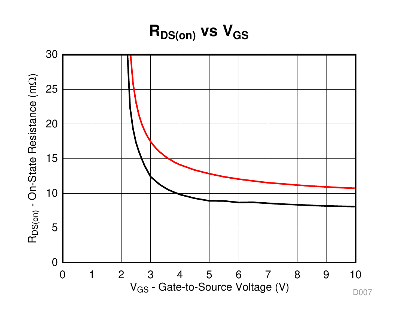
\includegraphics[width=0.6\textwidth]{Chapters/Figures/chapter3/CSD17308Q3_rdson.pdf}
	\caption{$R_{DS(ON)}$ on-state resistance (m$\Omega$) as a function of the $V_{GS}$ gate-to-source voltage (V), for the CSD17308Q3 power MOSFET~\cite{CSD17308Q3}.}
	\label{fig:CSD17308Q3_rdson}
\end{figure}
\begin{figure}[h]
	\centering
	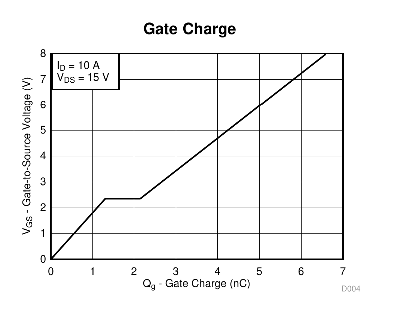
\includegraphics[width=0.6\textwidth]{Chapters/Figures/chapter3/CSD17308Q3_gate_charge.pdf}
	\caption{$V_{GS}$ gate-to-source voltage (V) as a function of the $Q_G$ gate charge (nC), for the CSD17308Q3 power MOSFET~\cite{CSD17308Q3}.}
	\label{fig:CSD17308Q3_gate_charge}
\end{figure}

According to Figure~\ref{fig:CSD17308Q3_crss} taken from~\cite{CSD17308Q3}, the reverse transfer capacitance ($C_{RSS}$, also known as Miller capacitance) for a $V_{DS}$ of 15V in the CSD17308Q3 model is, typically, 27pF, which is about half of this same measure for the Si7212DN model (measured at around 50pF, visible on the graph of Figure~\ref{fig:Si7212DN_crss}). $C_{RSS}$ corresponds to the gate-to-drain parasitic capacitance ($C_{gd}$), and therefore it is important for its value to be as low as possible, in order to reduce gain losses when working with high frequency values -- clearly the case for the PWM operating frequency.

%tentar juntar as duas figuras lado a lado!!!!!!!
%meter imagem CSD17308Q3_crss:
\begin{figure}[h]
	\centering
	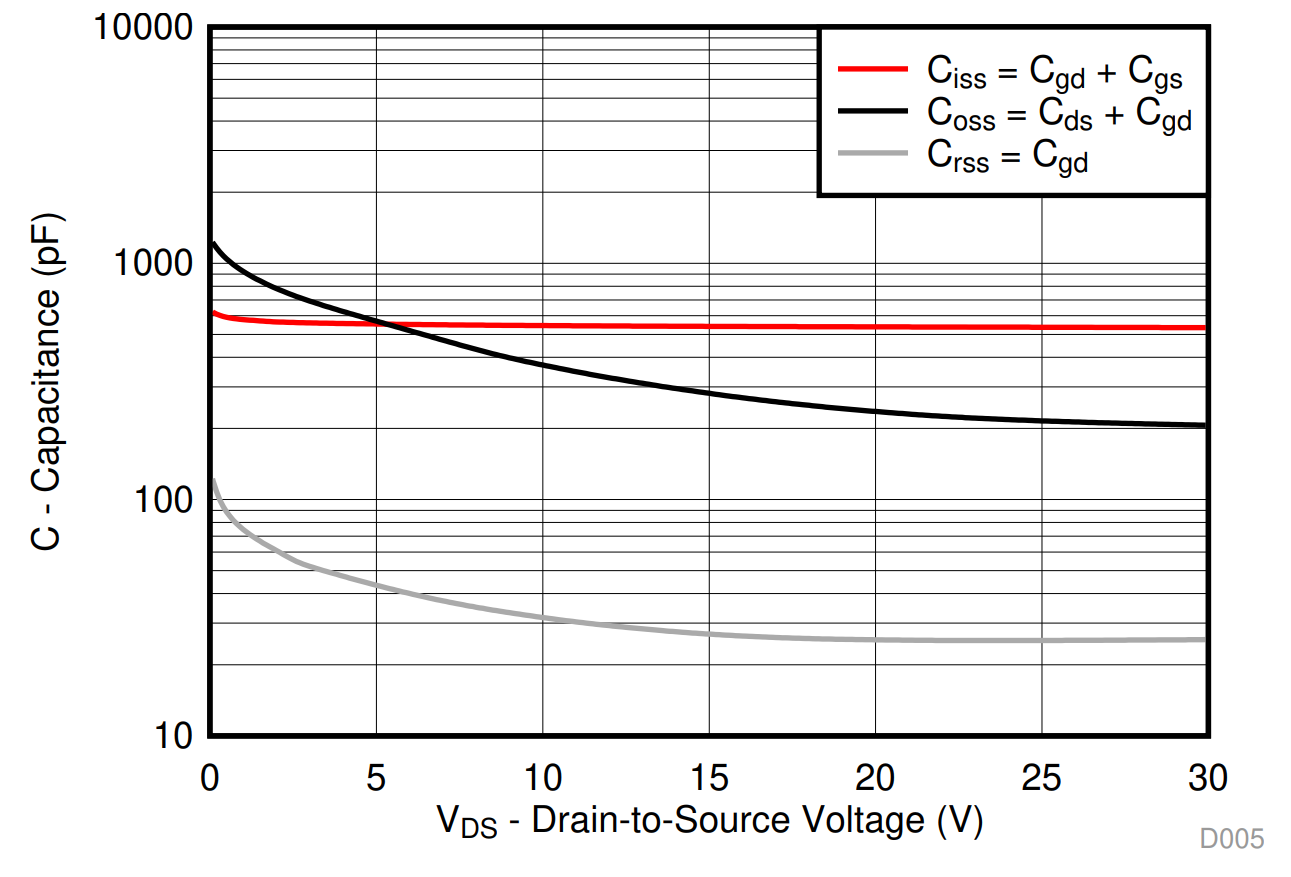
\includegraphics[width=0.5\textwidth]{Chapters/Figures/chapter3/CSD17308Q3_Crss.png}
	\caption{$C_{RSS}$ reverse transfer capacitance for the CSD17308Q3 power MOSFET~\cite{CSD17308Q3}.}
	\label{fig:CSD17308Q3_crss}
\end{figure}
%meter imagem Si7212DN_crss:
\begin{figure}[h]
	\centering
	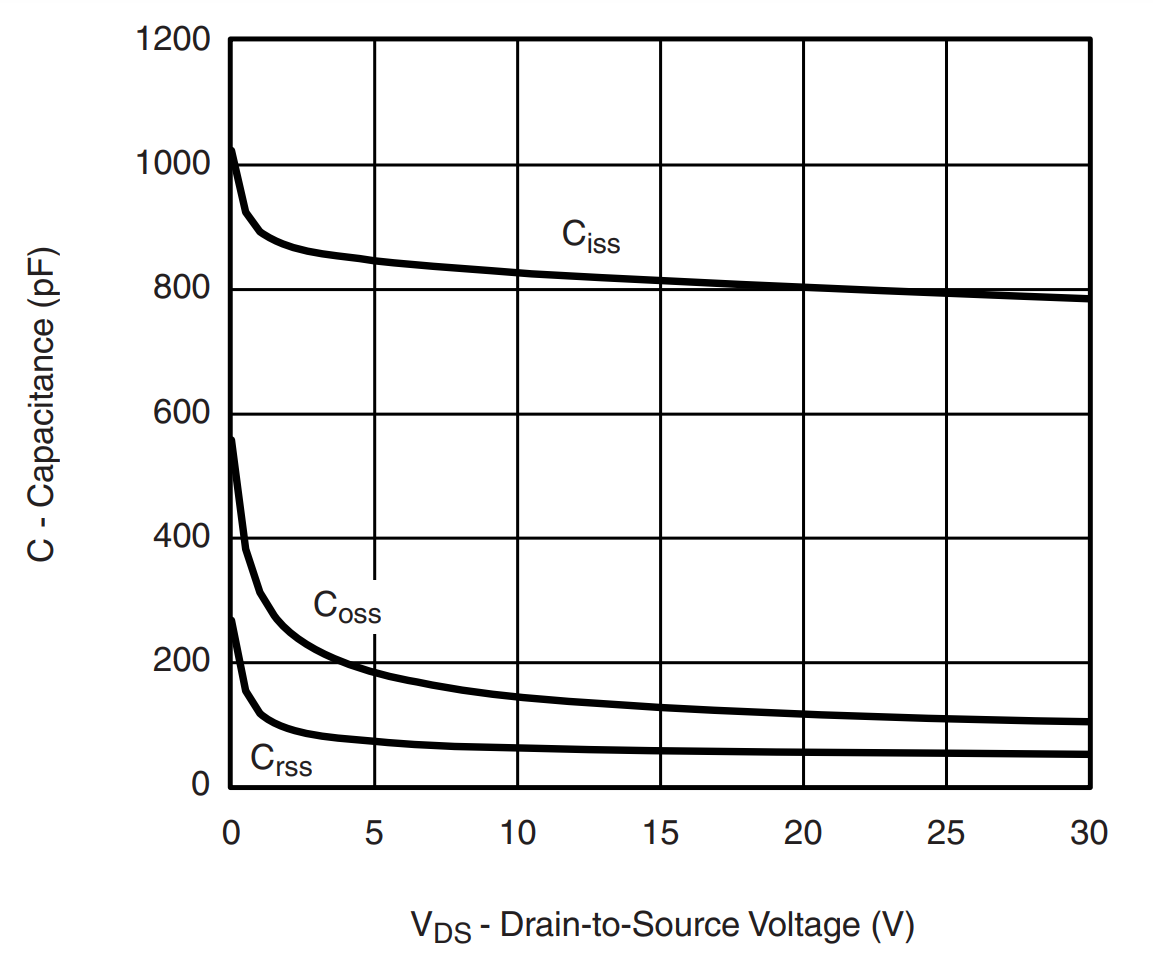
\includegraphics[width=0.5\textwidth]{Chapters/Figures/chapter3/Si7212DN_Crss.png}
	\caption{$C_{RSS}$ reverse transfer capacitance for the Si7212DN power MOSFET~\cite{Si7212DN}.}
	\label{fig:Si7212DN_crss}
\end{figure}

Regarding the $B_{V_{DSS}}$ maximum rated drain-source voltage -- also known as the reverse breakdown voltage --, there is not a particularly advatageous FET to be chosen, since this value is equal for both models, sitting at 30V. It also comfortably exceeds the projected $V_{CLP}$ maximum of 15V.

Finally, when it comes to the devices' actual switching characteristics, namely time-related, the CSD17308Q3 model once again trumps the Si7212DN model, since both the turn-on and turn-off delay times ($t_{d(ON)}$ and $t_{d(OFF)}$, respectively), as well as the rise time ($t_r$), never typically surpass double digits for the substituting model, whereas those same specifications are substantially higher for the suggested model.

The selection of the CSD17308Q3 MOSFET can thus be looked forward to as the switch FET for the buck converter topology~\cite{LTC4012,CSD17308Q3,Si7212DN}.

%---------------------
%%	EXPLICAR AQUI neste paragrafo a seguir! COMO FUNCIONA BOOTSTRAPPING
%% NUM CONVERSOR DC/DC
%%
%%        *****     I M P O R T A N T E     *****     
%%                       BOOTSTRAP

%% NESTE CASO, O datasheet DO LTC4012 NAO EXPLICA O FUNCIONAMENTO DO BOOTSTRAPPING, APENAS MENCIONA QUE EXISTE E OS DIODOS E CONDENSADORES A USAR. FOI ISSO QUE METI AQUI neste parágrafo.

%------------------------
% usar isto que está aqui para explicar o BOOTSTRAP:
% -- the aforementioned 
% SW (Pin 18): PWM Switch Node. The LTC4012 uses the
% voltage on this pin as the source reference for its topside
% NFET (PWM switch) driver.

% TGATE (Pin 19): External NFET Switch Gate Control Output.
% This output provides gate drive to an external NMOS power
% transistor switch used in the DC/DC converter. Operating
% voltage range is GND to (CLN + 5V).

% BGATE (Pin 16): External Synchronous NFET Gate Control
% Output. This output provides gate drive to an external NMOS
% power transistor switch used for synchronous rectification
% to increase efficiency in the step-down DC/DC converter.
% Operating voltage is GND to INTVDD. BGATE should be
% left floating if not used.

% INTVDD (Pin 17): Internal 5V Regulator Output. This pin
% provides a means of bypassing the internal 5V regulator
% used to power the LTC4012 PWM FET drivers. This supply
% shuts down when the LTC4012 shuts down. Refer to the
% Application Information section for details if additional
% power is drawn from this pin by the application circuit.

% BOOST (Pin 20): TGATE Driver Supply Input. A bootstrap
% capacitor is returned to this pin from a charge network
% connected to SW and INTVDD. Refer to the Applications
% Information section for complete details on circuit topology
% and component values. Operating voltage ranges from
% (INTVDD - 1V) to (CLN + 5V).
%------------------------

%							PAREI AQUI!!!!!!!!!!!!!!!!!!

							% a cena do BOOTSTRAP tem de entrar depois do \paragraph. Depois posso começar a dizer o que ja está aqui. Exemplo: *BOOTSTRAP EXPLICAÇAO breve*. The LTC4012 offers the possibility...
\paragraph{The TGATE BOOST Supply and Diode Selection}	The LTC4012 offers the possibility of assembling a bootstrapped supply on the BOOST input pin (pin 20), for the 19th pin of the IC, TGATE. The latter is an output dedicated to the gate control of the external N-channel power switch (Q2 from Figure~\ref{fig:LTC4012_circuit}) used for the step-down DC/DC conversion. The bootstrapping is fully established with the connection of a capacitor and a Schottky diode to the BOOST pin, represented by components C4 and D3 in Figure~\ref{fig:LTC4012_circuit}, respectively, as well as a second capacitor, C6, connected between the INTVDD pin and GND. The C4 capacitor's value can be determined through expression (\ref{eq:c4_cap}),

\begin{equation}\label{eq:c4_cap}
	C4=\frac{20 \cdot Q_G}{4.5\textrm{V}}\,,\medskip
\end{equation}
from which the C6's value is calculated:

\begin{equation}\label{eq:c6_cap}
	C6=20 \cdot C4\,\medskip
\end{equation}

\noindent For expression (\ref{eq:c4_cap}), $Q_G$ refers to the rated gate charge for the CSD17308Q3 power FET, for $V_{GS}=4.5$V; after referring once again to Figure~\ref{fig:CSD17308Q3_gate_charge}, approximately 17nF result for C4. C6 will therefore be valued at approximately $0.35 \mu$F. Referring to the INTVDD pin, which corresponds to the internal 5V regulator output, the LTC4012 application information suggests a bypass of this regulator with a ceramic capcitor to GND; a value of $0.47 \mu$F or larger is suggested. The original application information's capacitor suggestions for the bootstrapped BOOST pin's components were therefore taken. Higher values than the ones calculated for both C4 and C6 capacitors were used, namely $\textrm{C4}=0.1 \mu$F and $\textrm{C6}=2 \mu$F. C6 also serves as the ceramic bypass capacitor of the INTVDD regulator output.
%explicar pq é que nao faz mal meter C4=0.1uF e C6=2uF...

The Schottky diode selected for D3 was the CMDSH-3 model suggested by the LTC4012 datasheet, and it is connected between pins BOOST and INTVDD.
The use of such diode increases the $V_{GS}$ voltage applied to the top FET, since the forward voltage drop on these components tends to be lower when compared with silicon diodes.
This specification allows the diode to consume less power, dissipating less heat, and therefore it is a more efficient way to block the reverse flow of current, also subsequently improving the converter's efficiency itself.

The use of another diode is necessary, this time in parallel with the bottom FET, being a Schottky model again advised. Besides the lower power consumption, this type of diode has a fast reverse recovery time, which present an advantage when used in fast switching applications. It is represented in the circuit of Figure~\ref{fig:LTC4012_circuit} by D4. The suggested model by the typical application circuit present in the LTC4012 datasheet is the MBR230LSFT1, but at the component selection phase, it was unavailable, and therefore the similar SS34FA model was selected. It should be noted that this Schottky diode presents an extra advantage, as it was designed to have an $I_R$ reverse current of $500 \mu$A, half of the same specification for the MBR230LSFT1 model.

Lastly, the placement of a final Schottky diode is also advised between the system power node (i.e. the PWR\_SUPPLY net) and the BAT pin of the LTC4012 (i.e. the VBAT net). This diode is intended as a means to prevent the flow of current from the external power adapater to the battery terminal, while also aiding in the powering of the load applied to the subsequent circuit when said adapter is unconnected~\cite{LTC4012,CSD17308Q3}.

\paragraph{Loop Compensation and Soft-Start} %ler a partir de "Soft-Start" para entender os 3 loops de PWM -- pag. 12-15

The three separate PWM control loops of the LTC4012 (current, voltage or adapter limit) can be compensated by a single set of components attached between the ITH pin and GND. As shown in the typical LTC4012 application, a 6.04k resistor in series with a capacitor of at least 0.1uF provides adequate loop compensation for the majority of applications.
The LTC4012 can be soft-started with the compensation capacitor on the ITH pin. At start-up, ITH will quickly rise to about 0.25V, then ramp up at a rate set by the compensation capacitor and the 40uA ITH bias current.
The full programmed charge current will be reached when ITH reaches approximately 2V. With a 0.1uF capacitor, the time to reach full charge current is usually greater than 1.5ms.
This capacitor can be increased if longer start-up times are required, but loop bandwidth and dynamic response will be reduced~\cite{LTC4012}.

%s--Ss--Ss--Ss--Ss--Ss--Ss--Ss--Ss--Ss--Ss--Ss--Ss--Ss--Ss--Ss--Ss--Ss--Ss--S

\subsubsection{Battery Balancer}\label{sec:3212_BQ29209}

The battery pack used for this project relies on two equal Li-ion cells disposed in a 2-Series cell configuration, which imperatively requires cell balancing -- a specific technique used for preserving the batteries' health, i.e. their life cycle. Although the two cells used for the backup pack are the same model, there will certainly be discrepancies between them, since no two batteries are the same, which translates in different levels for the \gls{SoC} of both cells. Such problem requires a way not to allow the draining of any cell below its rated cut-off voltage (in the case of the INR18650-35E cell, 2.65V, as presented in Table~\ref{tab:battery2S}) or overcharging past the 4.20V ($\pm0.05$V) termination voltage limit. Texas Instruments offers a low-power solution for this: the BQ29209 is an IC capable of providing automatic cell balance for 2-series cell Li-ion battery packs, along with overvoltage protection. The cell balancing is achieved through the comparison of each cell's voltage, enabling and disabling the feature when nominal differences of 30mV (or more) or 0mV, respectively, are detected.

BQ29209's datasheet (\cite{bq29209}) provides a typical application circuit, as well as some application notes. However, the typical application circuit cannot be implemented for the new beRTK\textsuperscript{\textregistered}, since the internal system of this battery balancer can only support cell balancing currents of up to 15mA, which would not cause any kind of reaction within the INR18650-35E cells used, since their minimum charge current is 68mA. Therefore,~\cite{bq29209} provides an application circuit capable of supporting a cell balancing current higher than 15mA, which was adapted for this project. This implementation is presented in Figure~\ref{fig:BQ29209_circuit}. %caso meta esta parte, descomentar o minimum charge current de 68mA da Table 3.1!

% meter aqui circuito do BQ29209
\begin{figure}[H]
    \centering
    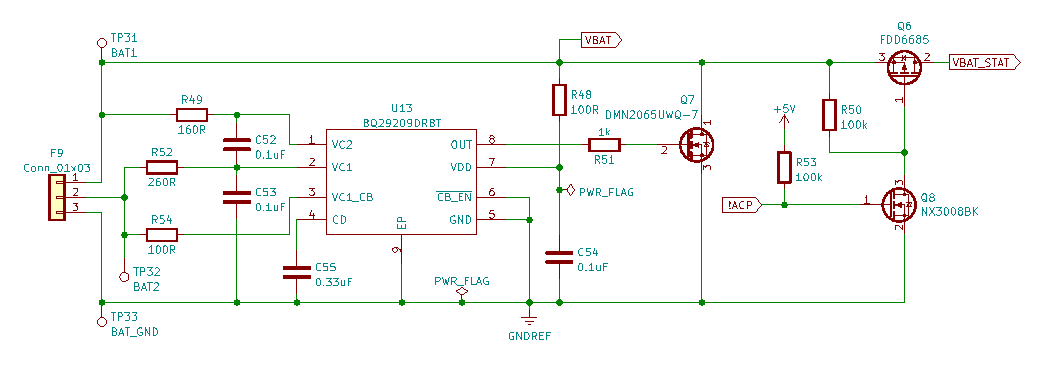
\includegraphics[width=1.0\textwidth]{Chapters/Figures/chapter3/Battery_Balancer.pdf}
    \caption{beRTK\textsuperscript{\textregistered} Base Station's Battery Balancer schematic diagram.}
    \label{fig:BQ29209_circuit}
\end{figure}

The circuit of Figure~\ref{fig:BQ29209_circuit} is valid for a $V_{DD}$ supply voltage that ranges from 4V to 10V. In this case, the BQ29209 IC is powered by the battery pack, and therefore $V_{DD}$ is approximately equal to the battery pack's voltage (due to the 100$\Omega$ R48 resistor), which will always be maintained within the intended voltage supply range. This same circuit also ensures that, due to FETs Q3 (NMOS) and Q10 (PMOS), a higher cell balancing current can safely be established, being it defined by either cell's voltage, along with resistor R4:

\begin{equation}\label{eq:IBAL}
	I_{BAL}=\frac{V_{Cell}}{R4}\,\medskip
\end{equation}

\noindent It should be noted that resistor R54's purpose lies on ensuring that both ``balancing'' FETs will remain off while cell balancing is not taking place and should be selected with a value above 2k$\Omega$.

\cite{bq29209} clarifies that the BQ29209 ensures cell balancing on the cell that presents the higher voltage of the pack.
Taking into account that recommended cell arrangement sequence (from the bottom of the stack) of GND--Cell1--Cell2 (i.e. from pin 3 to pin 1 of connector F9 -- Figure~\ref{fig:BQ29209_circuit}) was followed, the balancing of Cell1 would start by pulling pin VC1\_CB of BQ29209 to GND, therefore setting PMOS Q10's gate-source voltage at around $-V_{Cell1}$. This would cause a balancing current of $I_{BAL1}=\frac{V_{Cell1}}{R4}$. Conversely, if Cell2 were in need of balancing, VC1\_CB would instead be pulled to $V_{DD}$, thus setting Q3's gate voltage at around $V_{Cell1}+V_{Cell2}$, which translates into a gate-source voltage of approximately $V_{Cell2}$, having the source voltage being set at around $V_{Cell1}$. With this, resorting again to equation (\ref{eq:IBAL}), a cell balancing current of $I_{BAL2}=\frac{V_{Cell2}}{R4}$ results. In order to set a balancing current for each cell that would always surpass the minimum charge current of 68mA, a value of 20$\Omega$ was sized for R4. 

The remaining components' values were selected as to comply with the BQ29209 recommended operating conditions, except for the delay time capacitance, C55, which can be calculated based on a desired delay time ($t_d$) for the activation of the overvoltage protection feature -- expression (\ref{eq:CCD}) --, as well as on an overvoltage delay time scale factor, $X_{DELAY}$, expressed in $s/ \mu F$.

\begin{equation}\label{eq:CCD}
	C55=\frac{t_d}{X_{DELAY}}\,\medskip
\end{equation}

\noindent As the nominal value for $X_{DELAY}$ is $9s/ \mu$F, a delay time capacitance of $0.33 \mu$F results.

It must be noted that the overvoltage protection feature is not indicated for the project's backup battery pack, since due to each cell's charging cycle termination voltage limit being 4.20V, this level will not meet the only two fixed overvoltage protection thresholds rated for the BQ2920x product family (4.30V or 4.35V, $\pm 0.25$mV) without causing damage overtime. Nevertheless, the delay time capacitance is still included in the circuit, for a future version of the beRTK\textsuperscript{\textregistered} with different backup battery pack specifications. Also concerning the overvoltage feature is the OUT output pin component setting, composed by a resistor and a MOSFET (R51 and Q7, respectively). The OUT output pin is initially set low, only switching to a high state when any cell reaches an overvoltage condition. This high state activates MOSFET Q7, shunting the battery power supply to ground in order to preserve health and life cycle of the cells.

Regarding the indication of the state of the battery pack's voltage, MOSFETs Q6 and Q8 make up another switching system as the one presented in Section~\ref{sec:3213_SWITCH}, for the Power Switch circuit. Observing once more Figure~\ref{fig:BQ29209_circuit}, it can be seen that the VBAT net is constantly supplying the battery pack's voltage through resistor R50 to Q6's gate. Being Q6 a P-channel type MOSFET, it will act as an open switch when such voltage is fed to its gate. This will not allow the battery pack's voltage to be transferred to net VBAT\_STAT, a net intended to supply a comparator used to indicate the status of this same voltage (hereby defined as the ``status voltage'') -- explained in Section~\ref{sec:3231_BACKPANEL}. This status voltage is only fed to the voltage comparator of Figure~\ref{fig:HMI_circuit} (U6) upon the activation of MOSFET Q8 of the BQ29209 circuit (Figure~\ref{fig:BQ29209_circuit}). Assuming the battery pack is connected to the system, Q8 can be arbitrarily turned off or on, just by plugging in or out the external power adapter, respectively. In other words, when only the adapter is not connected, Q8 will be on, and therefore Q6 will be on as well. Conversely, upon plugging the external adapter in, the LTC4012's $\overline{\mbox{ACP}}$ open-drain output will be pulled to GND, turning both Q8 and Q6 off, disabling the feeding of comparator U6 with the status voltage of the battery pack~\cite{bq29209}.

%s--Ss--Ss--Ss--Ss--Ss--Ss--Ss--Ss--Ss--Ss--Ss--Ss--Ss--Ss--Ss--Ss--Ss--Ss--S

\subsubsection{Power Switch}\label{sec:3213_SWITCH}

The circuit in charge of switching the system's power on and off is represented in Figure~\ref{fig:SWITCH_circuit}. Its function relies on an output signal set by a SN74LVC2G74DCTR, a D-type flip-flop -- manufactured by Texas Instruments~\cite{SN74LVC2G74DCTR} -- which in turn allows or blocks the incoming power from either the external power adapter or the battery pack (i.e. from the PWR\_SUPPLY net) to the voltage converter (Section~\ref{sec:3214_AP64501}) that powers the rest of the system.
This flip-flop output signal is, in turn, controlled by a push-button located on the outside of the base station casing, and when pressed ties the GND net to the input pin of a single Schmitt-trigger inverter -- 74AHC1G14, by Diodes Incorporated~\cite{74AHC1G14}.
Since this inverter's supply voltage pin (pin 5 of 74AHC1G14) is connected to the output of a low dropout voltage regulator (LDO) -- MCP1790, by Microchip~\cite{MCP1790} --, its output voltage will be, when driven low, that same output voltage; in this case, it will be equal to 5V.
With this, a positive voltage impulse is established on the CLK pin of the SN74LVC2G74DCTR, and since it relies on a single positive-edge-triggered architecture, it is activated, setting Q output to a high state, as per Table~\ref{tab:SN74LVC2G74DCTR}, driving the gate of the Q5 NMOS and subsequently shunting Q4 PMOS's gate to GND, driving it as well.
This opens a path for power from the mentioned PWR\_SUPPLY net to flow to the main 5V voltage regulator's input (the AP64501), i.e. to the PWR\_AP64501 net. When in this state, once the switch is pressed again, the flip-flop's Q output is set to low, successively shutting down both Q5 and Q4 MOSFETs, blocking the passage of power and thus shutting down the system.

% meter aqui circuito do Power SWITCH:
\begin{figure}[h]
    \centering
    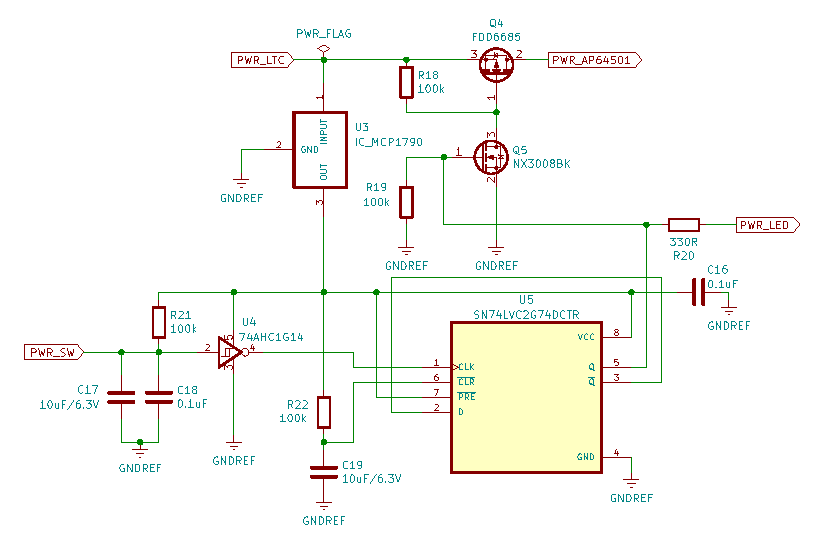
\includegraphics[width=1.0\textwidth]{Chapters/Figures/chapter3/Power_Switch.pdf}
    \caption{beRTK\textsuperscript{\textregistered} Base Station's Power Switch schematic diagram.}
    \label{fig:SWITCH_circuit}
\end{figure}

% FAZER ESTA TABELA (seguir https://tex.stackexchange.com/questions/210232/center-text-over-multicolumn-in-table)
\begingroup
\begin{table}[h]
    \caption{SN74LVC2G74 functional modes~\cite{SN74LVC2G74DCTR}.}
    \label{tab:SN74LVC2G74DCTR}
    \centering%@{}l@{}@{}c@{}@{}c@{}@{}c@{}@{}c@{}
    % \setlength{\tabcolsep}{10pt} % Default value: 6pt
    % \renewcommand{\arraystretch}{1.5} % Default value: 1
    \begin{tabular}{cccccccc}
        \toprule
		
		\multicolumn{4}{c}{\textbf{Inputs}} &&& \multicolumn{2}{c}{\textbf{Outputs}} \\
        \midrule
        $\mathbf{\overline{\mbox{\textbf{PRE}}}}$ & $\mathbf{\overline{\mbox{\textbf{CLR}}}}$ & \textbf{CLK} & \textbf{D} &&& \textbf{Q} & $\mathbf{\overline{\mbox{\textbf{Q}}}}$ \\
        \midrule
		L & H & X & X &&& H & L \\
		\midrule
		H & L & X & X &&& L & H \\
		\midrule
		L & L & X & X &&& H & H \\
		\midrule
		H & H & $\uparrow$ & H &&& H & L \\
		\midrule
		H & H & $\uparrow$ & L &&& L & H \\
		\midrule
		H & H & L & X &&& Q$_0$ & $\overline{\mbox{Q$_0$}}$ \\
        \bottomrule
    \end{tabular}
\end{table}
\endgroup
% parei aqui

% REFERÊNCIA needed!!!!!!!!!!!!!!!!!!!! ~SN74LVC2G74DCTR

%s--Ss--Ss--Ss--Ss--Ss--Ss--Ss--Ss--Ss--Ss--Ss--Ss--Ss--Ss--Ss--Ss--Ss--Ss--S

\subsubsection{Voltage Converter}\label{sec:3214_AP64501}

Most of the main ICs and many other components of the base station run on 5V. The best way to achieve such continuous supply level in this project is through the use of a DC-to-DC buck converter. The AP64501 (by Diodes Incorporated) synchronous buck converter was the selected part to establish the necessary 5V power source. High power efficiency can be achieved at light loads -- the case for the beRTK\textsuperscript{\textregistered} system --, since this device operates in \gls{PFM} mode. The operation occurs at a typical frequency of 570kHz. Upon heavy load supply needs, it operates in a forced PWM mode.

The AP64501 is capable of supplying DC voltage from 0.8V to 39V, as well as up to 5A of continuous current, for an input supply voltage ranging from 3.8V to 40V. It generates a low amount of quiescent current as well\footnote[11]{In a no-load and non-switching condition, the quiescent current typically generated by the AP64501 is $25 \mu$A.}, very important since this IC draws its power from either the external power adapter or the battery pack (via the LTC4012, i.e. the PWR\_SUPPLY net, as mentioned in Section~\cite{sec:3213_SWITCH}); a higher quiescent current could result in a non-negligible and unnecessary drain of the battery pack, while the system is in a stand-by/idle operation.

Similar to previously mentioned ICs, the AP64501's datasheet (\cite{AP64501}) also provides a typical application circuit, along with helpful application notes. These guidelines were adapted in order to construct the circuit displayed in the schematic of Figure~\ref{fig:AP64501_circuit}.

% meter aqui circuito do AP64501
\begin{figure}[h]
	\centering
	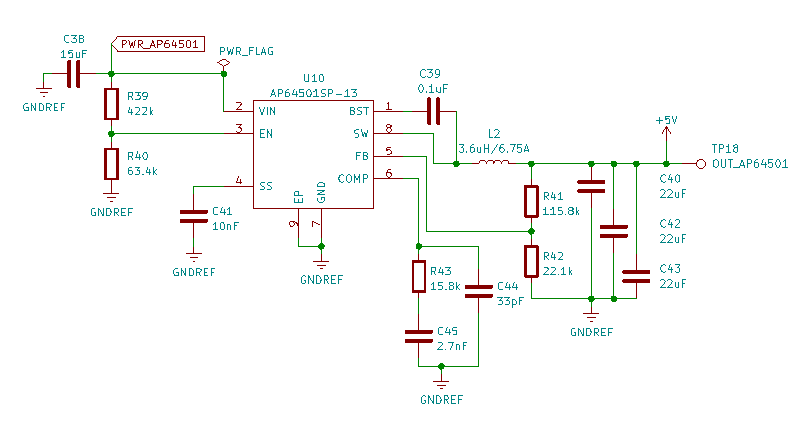
\includegraphics[width=1.0\textwidth]{Chapters/Figures/chapter3/Voltage_Converter.pdf}
	\caption{beRTK\textsuperscript{\textregistered} Base Station's Voltage Converter schematic diagram.}
	\label{fig:AP64501_circuit}
\end{figure}

The device starts operating as soon as the voltage applied to the EN (Enable) pin is greater than its logic high threshold -- typically 1.18V. This pin can also be used to program a feature of \gls{UVLO}, or be tied directly to the voltage input pin (VIN) to start up automatically as the voltage on that pin increases. This start-up should not be abrupt, due to the possibility of output voltage overshoot and inrush current problems, and therefore the AP64501 offers the possibility of programming a soft-start time via a recommended 10nF capacitor, represented by C41 in Figure~\ref{fig:AP64501_circuit}. The value for this capacitor can be determined through expression (\ref{eq:C41}),

\begin{equation}\label{eq:C41}
	C41 = 5.3 \cdot t_{ss}\,,\medskip
\end{equation}
where C41 is the capacitance (in nF) and must be at least equal to 10nF, and $t_{ss}$ is the soft-start time (in ms) and must be at least 4ms. Therefore, if a higher soft-start time is desired, a simple tweak in the $t_{ss}$ variable will yield a new soft-start capacitor value.

\paragraph{Programming the UVLO}	The AP64501 offers a default UVLO setting for when insufficient supply voltages are detected by an internal UVLO comparator; the default is set for when the supply falls below 3.1V. However, if a higher UVLO voltage is required by the application, it can be set through a voltage divider centred around the EN pin (Figure~\ref{fig:UVLO_divider}).

\begin{figure}[h]
	\centering
	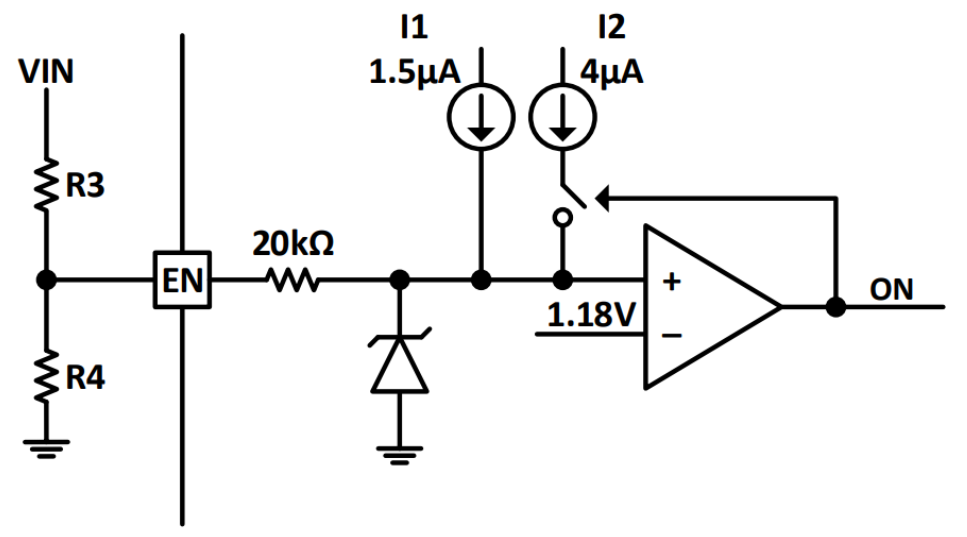
\includegraphics[width=0.5\textwidth]{Chapters/Figures/chapter3/UVLO.png}
	\caption{Voltage divider used to program the UVLO feature of the AP64501~\cite{AP64501}.}
	\label{fig:UVLO_divider}
\end{figure}

Figure~\ref{fig:UVLO_divider} presents the external voltage divider setting that can be implemented in order to program the UVLO feature, where resistors R3 and R4 correspond to resistors R10 and R13 (respectively) of Figure~\ref{fig:AP64501_circuit}. The values of such resistors can be determined through expressions (\ref{eq:R10}) and (\ref{eq:R13}):

\begin{equation}\label{eq:R10}
	R10 = \frac{0.924 \cdot V_{ON} - V_{OFF}}{4.1 \mu \textrm{A}}\,\medskip
\end{equation}

\begin{equation}\label{eq:R13}
	R13 = \frac{1.09 \cdot R10}{V_{OFF} - 1.09 \textrm{V} + 5.5 \mu \textrm{A} \cdot R10}\,\medskip
\end{equation}

Where:
\begin{itemize}
	\item $V_{ON}$ -- Rising edge VIN voltage required to enable the regulator. Must be greater than 3.7V;
	\item $V_{OFF}$ -- Falling edge VIN voltage required to disable the regulator. Must be greater than 3.3V.
\end{itemize}

In the case of this project, each battery cell has a discharge cut-off voltage of 2.65V, which corresponds to a total battery pack discharge cut-off voltage of around 5.3V. Therefore, a value greater than 5.3V should be chosen for $V_{OFF}$, in order to account for the preservation of the battery pack. Let this value be 5.5V.

The $V_{ON}$ voltage to enable the regulator must be chosen considering the possibility of the system powered on by the battery pack only. This pack's maximum voltage will not surpass 8.4V, and therefore $V_{ON}$ must be lower than that. Also considering the likeliness of the battery pack not being fully charged at the time on powering on the system, 6V would a safe low value for $V_{ON}$.

% apresentar os resultados do excel:
Substituting the $V_{ON}$ and $V_{OFF}$ in (\ref{eq:R10}), $10.732$k$\Omega$ result for R10. Subsequently, using this value in (\ref{eq:R13}), $2.617$k$\Omega$ result for R13. The closest values available for R10 and R13 at the prototyping phase were 11k$\Omega$ and 2.7k$\Omega$, respectively. Reversing expressions (\ref{eq:R10}) and (\ref{eq:R13}) and using these adapted resistor values result in the intended $V_{ON}$ and $V_{OFF}$ values.

As stated in the last paragraph of Section~\ref{sec:313_PowerSupply}, the input voltage of the system (and therefore the input voltage of the LTC4012) can range from 15V to 22V. It should then be added that if the system is supplied with a maximum of 22V (by the external adapter), the AP64501 is still turned on, since that value lies well within the EN pin voltage rating. Therefore, even in this case, the UVLO feature will still be available.

\paragraph{Setting the Output Voltage}	As stated earlier, the AP64501 is able to output voltages that range from 0.8V to 39V. For this project, in order to program the desired 5V output voltage, once again a voltage divider is used. This simple double-resistor setup is composed by R41 and R42, whose values can be determined solely from expression (\ref{eq:R41_R42}):

\begin{equation}\label{eq:R41_R42}
	R41 = R42 \cdot \left(\frac{V_{OUT}}{0.8 \textrm{V}} - 1\right)\,\medskip
\end{equation}

\cite{AP64501} provides a table with recommended values for the components to select for various fixed output voltage values, in order to construct the typical application circuit of the AP64501. Such table is represented by Table~\ref{tab:AP64501_recommended_values}. According to (\ref{eq:R41_R42}), for an output voltage of 5V (i.e. $V_{OUT} = 5$V), fixating $\textrm{R42} = 22.1 \textrm{k}\Omega$ results in a value of around 116k$\Omega$ for R41. A standard resistor value close to this would be 115.8k$\Omega$, which can be confirmed by Table~\ref{tab:AP64501_recommended_values}.

\begingroup
\begin{table}[h]
    \caption{AP64501 recommended component values, for several fixed $V_{OUT}$ output voltages (adapted from~\cite{AP64501}).}
    \label{tab:AP64501_recommended_values}
    \centering%@{}l@{}@{}c@{}@{}c@{}@{}c@{}@{}c@{}
    % \setlength{\tabcolsep}{10pt} % Default value: 6pt
    % \renewcommand{\arraystretch}{1.5} % Default value: 1
	\begin{tabular}{cccccccccc}
        \toprule
        $\mathbf{V_{OUT}}$ & \textbf{R41} 						    & \textbf{R42} 							  & \textbf{L2} 						& \textbf{C38} 						  & $\mathbf{C_{OUT}}$ 					& \textbf{C39} 						  & \textbf{R43} 						   & \textbf{C45}  & \textbf{C44} \\
       	\textbf{(V)} 	   & \textbf{(k}$\mathbf{\Omega}$\textbf{)} & \textbf{(k}$\mathbf{\Omega}$\textbf{)}  & \textbf{(}$\mathbf{\mu}$\textbf{H)} & \textbf{(}$\mathbf{\mu}$\textbf{F)} & \textbf{(}$\mathbf{\mu}$\textbf{F)} & \textbf{(}$\mathbf{\mu}$\textbf{F)} & \textbf{(k}$\mathbf{\Omega}$\textbf{)} & \textbf{(nF)} & \textbf{(pF)} \\
        \midrule
		1.2 & 11.0 & 22.1 & 1.5 & 10& 3 x 22 & 0.1 & 3.74 & 2.7 & 150 \\
		\midrule
		1.5 & 19.6 & 22.1 & 2.2 & 10& 3 x 22 & 0.1 & 4.75 & 2.7 & 120 \\
		\midrule
		1.8 & 27.4 & 22.1 & 2.2 & 10& 3 x 22 & 0.1 & 5.62 & 2.7 & 100 \\
		\midrule
		2.5 & 47.5 & 22.1 & 3.3 & 10& 3 x 22 & 0.1 & 7.87 & 2.7 & 68 \\
		\midrule
		3.3 & 69.8 & 22.1 & 3.3 & 10& 3 x 22 & 0.1 & 10.50 & 2.7 & 56 \\
		\midrule
        5.0 & 115.8 & 22.1 & 3.6 & 10 & 3 x 22 & 0.1 & 15.80 & 2.7 & 33 \\
		\midrule
	    12.0 & 309.0 & 22.1 & 10.0 & 10 & 3 x 22 & 0.1 & 37.40 & 2.7 & 15 \\
		\bottomrule
	\end{tabular}
\end{table}
\endgroup

\paragraph{Selecting the Inductor}	Once again, the topic of inductor selection for a buck converter arises. The AP64501 relies on a pre-defined frequency in order to deliver the appropriate amount of power to the load connected upstream.
Switching the supply voltage on and off according to a certain duty cycle results in the sought-after 5V, and for that, a proper inductor is critical. It is recommended by \cite{AP64501} the selection of an inductor value between $1 \mu$H to $10 \mu$H, and therefore, taking into account the values presented in Table~\ref{tab:AP64501_recommended_values}, an inductor of $3.6 \mu$H was selected. It is also advised to select an inductor with a DC current rating of at least 35\% higher than the maximum 5A load current of the AP64501, which corresponds to 6.75A.

\cite{AP64501} also offers an equation to determine the L2 inductor value that can be used for most design applications -- represented by (\cite{eq:L2}).

\begin{equation}\label{eq:L2}
	L2 = \frac{V_{OUT} \cdot \left(V_{IN} - V_{OUT}\right)}{V_{IN} \cdot \Delta I_L \cdot f_{sw}}\,,\medskip
\end{equation}
where:
\begin{itemize}
	\item $\Delta I_L$ -- Inductor current ripple. Should be between 30\% to 50\% of the maximum load current the AP64501 is able to provide, which is 5A;
	\item $f_{sw}$ -- Buck converter typical oscillator frequency ($=570$kHz).
\end{itemize}

Note that there is a $0.1 \mu$F capacitor connecting the terminals switching and boost terminals of the device, SW and BST, respectively. the latter is used by the AP64501 in order to aid in the driving of the high-side power MOSFET. For that, the mentioned $0.1 \mu$F capacitor is recommended by~\cite{AP64501}.

\paragraph{Selecting the Input Capacitor}	Similarly to input capacitor selected for the LTC4012's +15VDC power input (DCIN), an input capacitor for the VIN pin the AP64501 must also be chosen. As stated before, this capacitor is tasked with the bypassing of switching noise from the device, as well as minimizing the impact of surge currents that arrive to its input terminal. Following once again Table~\ref{tab:AP64501_recommended_values} and the~\cite{AP64501} datasheet, it can be ascertained that an input capacitor value of at least $10 \mu$F is recommended. In this case, $15 \mu$F were used for this part.

\paragraph{Adjusting the Loop Compensation}	In order to adjust the loop response, an external RC network may be connected to the COMP pin of the device. This network is composed of resistor R43 and capacitor C45. Table~\ref{tab:AP64501_recommended_values} recommends 15.80k$\Omega$ and 2.7nF as the values for R43 and C45, respectively. The addition of an extra capacitor in parallel with the R43 and C45 series is able to cause an increase in the gain margin, as well as a decrease in phase margin. The recommended value is 33pF\footnote[12]{\cite{AP64501} dedicates a detailed section regarding the calculation of the COMP compensation pin's network.}.

\paragraph{Selecting the Output Capacitor}	Generally, filtering the switching noise generated by a buck converter can be done with the help of an inductor and a capacitor. This is applicable for the AP64501.
Observing once again Figure~\ref{fig:AP64501_circuit}, the last components to mention are the three output capacitors, represented by C40, C42 and C43. These capacitors all represent the same output capacitance, and therefore serve the same purpose, and for simplicity reasons, will be labelled as ``$C_{OUT}$''. The output capacitance on the AP64501 is charged with the typical decoupling capcitor tasks, among which are the filtering of unwanted noise, as mentioned several times before.
\cite{AP64501} presents an interesting approach: instead of using just a single output filtering capacitor, three of the same kind are suggested; Table~\ref{tab:AP64501_recommended_values} suggests using three $22 \mu$F capacitors -- in this case, in parallel.\footnote[13]{Naturally,~\cite{AP64501} also dedicated a section to the calculation of the ideal value for the $C_{OUT}$ capacitance, also mentioning that, for most applications, $22 \mu$F to $68 \mu$F ceramic output capacitors are acceptable.}.\\

With this, the 5V supply can be established. In the schematics of the system circuit -- displayed in present Chapter --, this supply is represented by a schematic symbol composed of a vertical arrow with a ``+5V'' label above it (observable on the right side of Figure~\ref{fig:AP64501_circuit}).


% VIN 2
% Power Input. VIN supplies the power to the IC as well as the step-down converter power MOSFETs. Drive VIN with a
% 3.8V to 40V power source. Bypass VIN to GND with a suitably large capacitor to eliminate noise due to the switching
% of the IC. See Input Capacitor section for more details.

% EN 3
% Enable Input. EN is a digital input that turns the regulator on or off. 
% Drive EN high to turn on the regulator and low to
% turn it off. Connect to VIN or leave floating for automatic startup. The EN has a precision threshold of 1.18V for
% programming the UVLO. See Enable section for more details.

% SS 4
% Soft-start. Place a ceramic capacitor from this pin to ground to program soft-start time. An internal 4μA current
% source pulls the SS pin to VCC. See Programming Soft-Start Time section for more details.
% FB 5
% Feedback sensing terminal for the output voltage. Connect this pin to the 
% resistive divider of the output.
% See Setting the Output Voltage section for more details.
% COMP 6

% Compensation. Connect an external RC network to the COMP pin to adjust the loop response. See External Loop
% Compensation Design section for more details.

% GND 7 Power Ground.

% SW 8
% Power Switching Output. SW is the switching node that supplies power to the output. Connect the output LC filter
% from SW to the output load.

% EXPOSED
% PAD 9
% Heat dissipation path of the die. The exposed thermal pad must be electrically connected to GND and must be
% connected to the ground plane of the PCB for proper operation and optimized thermal performance


% REFERÊNCIA needed!!!!!!!!!!!!!!!!!!!!

%sSsSsSsSsSsSsSsSsSsSsSsSsSsSsSsSsSsSsSsSsSsSsSsSsSsSsSsSsSsSsSsSsSsSsSsSsSsS

\subsection{Control}\label{sec:322_CONTROL}
	%mini introdução

%s--Ss--Ss--Ss--Ss--Ss--Ss--Ss--Ss--Ss--Ss--Ss--Ss--Ss--Ss--Ss--Ss--Ss--Ss--S
\subsubsection{CPU Board -- GPIO}\label{sec:3221_CM4_GPIO}

% meter aqui circuito do CM4_GPIO
\begin{figure}[h]
	\centering
	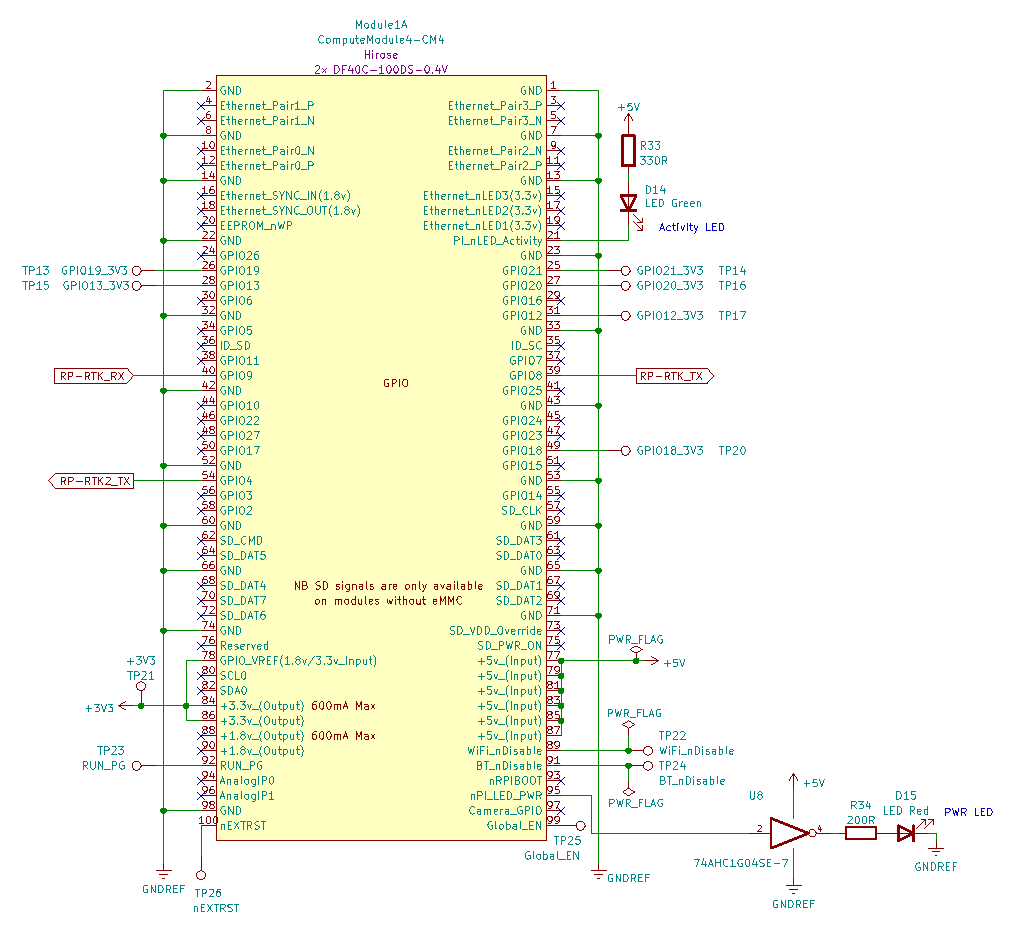
\includegraphics[width=1.0\textwidth]{Chapters/Figures/chapter3/CM4_GPIO.pdf}
	\caption{beRTK\textsuperscript{\textregistered} Base Station's CM4's GPIO schematic diagram.}
	\label{fig:CM4_GPIO_circuit}
\end{figure}

% REFERÊNCIA needed!!!!!!!!!!!!!!!!!!!!
%s--Ss--Ss--Ss--Ss--Ss--Ss--Ss--Ss--Ss--Ss--Ss--Ss--Ss--Ss--Ss--Ss--Ss--Ss--S

\subsubsection{CPU Board -- High-Speed}\label{sec:3222_CM4_HSpeed}

% meter aqui circuito do CM4_HighSpeed
\begin{figure}[h]
	\centering
	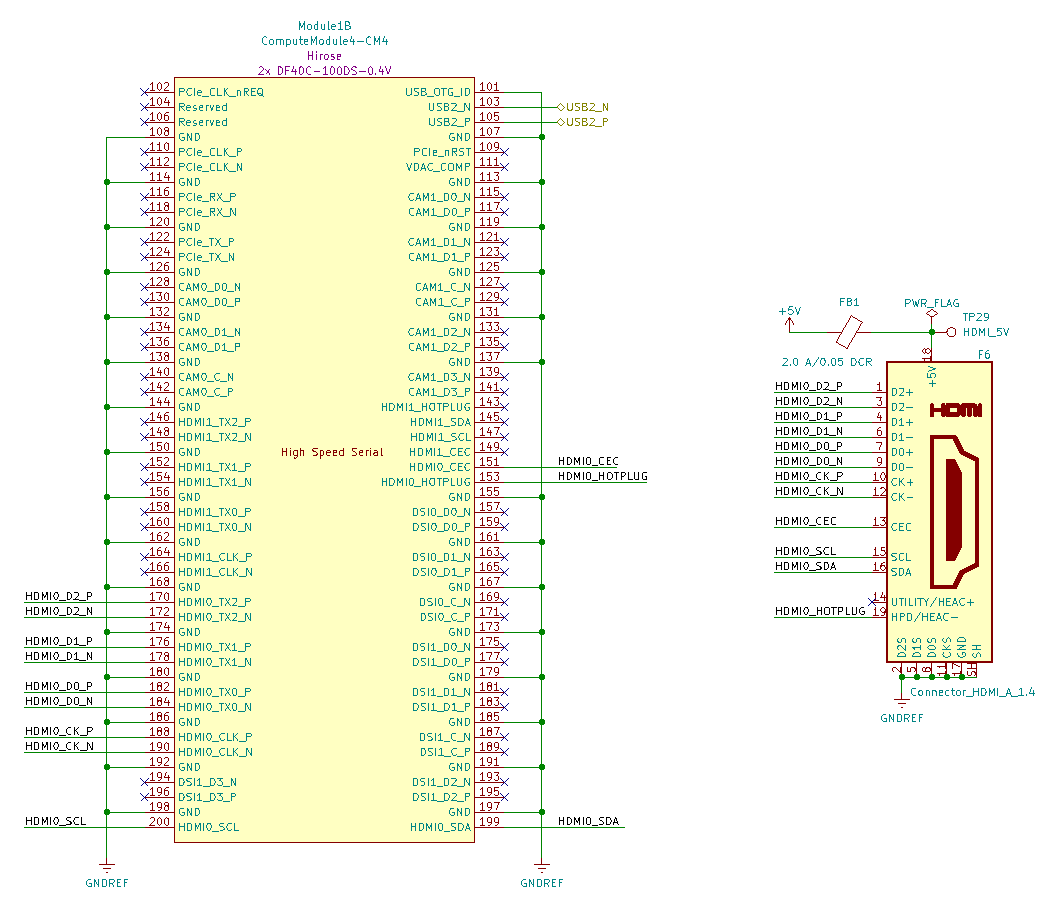
\includegraphics[width=1.0\textwidth]{Chapters/Figures/chapter3/CM4_HighSpeed.pdf}
	\caption{beRTK\textsuperscript{\textregistered} Base Station's CM4's High Speed schematic diagram.}
	\label{fig:CM4_HighSpeed_circuit}
\end{figure}

% REFERÊNCIA needed!!!!!!!!!!!!!!!!!!!!
%sSsSsSsSsSsSsSsSsSsSsSsSsSsSsSsSsSsSsSsSsSsSsSsSsSsSsSsSsSsSsSsSsSsSsSsSsSsS


\subsection{Peripherals and Communications}\label{sec:323_PERIPHERALS_COMMS}
	%mini introdução

%s--Ss--Ss--Ss--Ss--Ss--Ss--Ss--Ss--Ss--Ss--Ss--Ss--Ss--Ss--Ss--Ss--Ss--Ss--S

\subsubsection{Human-Machine Interface (HMI)}\label{sec:3231_BACKPANEL}

% meter aqui circuito do BACKPANEL
\begin{figure}[h]
	\centering
	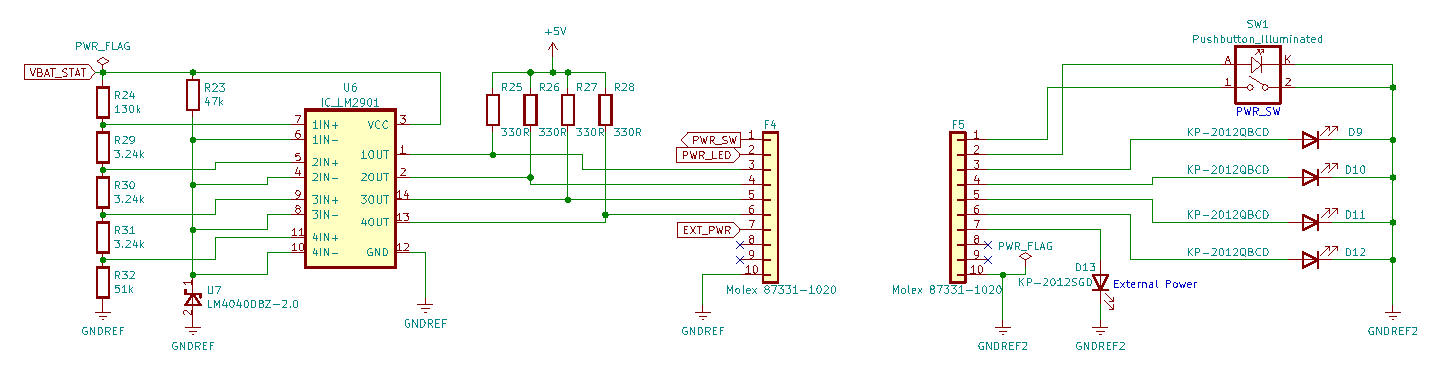
\includegraphics[width=1.0\textwidth]{Chapters/Figures/chapter3/Back_Panel.pdf}
	\caption{beRTK\textsuperscript{\textregistered} Base Station's HMI schematic diagram.}
	\label{fig:HMI_circuit}
\end{figure}

%https://www.farnell.com/datasheets/2702810.pdf - Diodo Zener 15V - explicar porque e que escolhi 15V...
%https://www.youtube.com/watch?v=GtH8lAzQf2A&ab_channel=GreatScott%21

% REFERÊNCIA needed!!!!!!!!!!!!!!!!!!!!

%s--Ss--Ss--Ss--Ss--Ss--Ss--Ss--Ss--Ss--Ss--Ss--Ss--Ss--Ss--Ss--Ss--Ss--Ss--S

\subsubsection{GNSS Receiver, RTK Radio Link and Wi-Fi Transceiver}\label{sec:3232_ZEDF9P_XBEE3}

% meter aqui circuito do ZEDF9P_XBEE3
\begin{figure}[h]
	\centering
	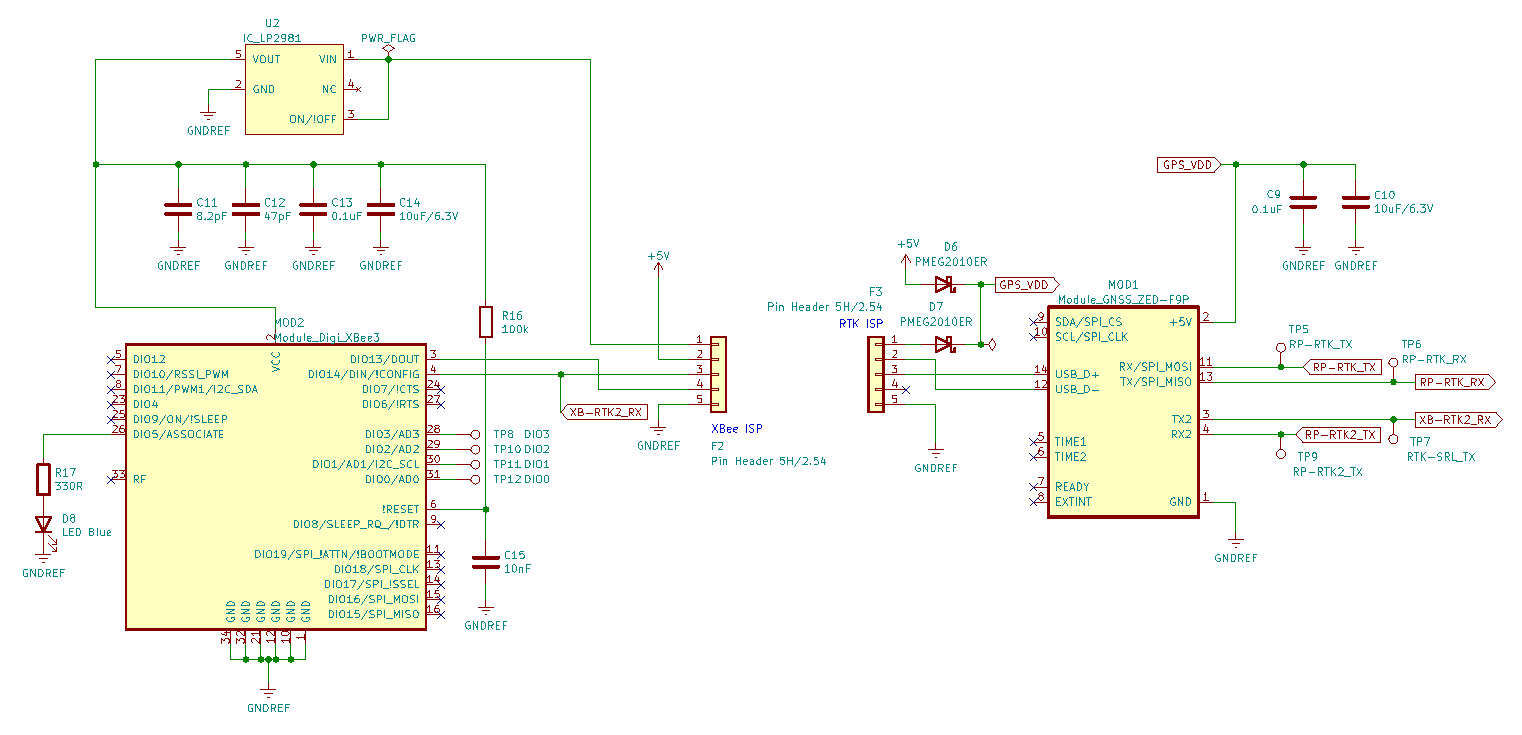
\includegraphics[width=1.0\textwidth]{Chapters/Figures/chapter3/Modules_ZEDF9P_XBEE3.pdf}
	\caption{beRTK\textsuperscript{\textregistered} Base Station's GNSS and Wi-Fi modules schematic diagram.}
	\label{fig:ZEDF9P_XBEE3_circuit}
\end{figure}

% REFERÊNCIA needed!!!!!!!!!!!!!!!!!!!!
%s--Ss--Ss--Ss--Ss--Ss--Ss--Ss--Ss--Ss--Ss--Ss--Ss--Ss--Ss--Ss--Ss--Ss--Ss--S

\subsubsection{USB Hub}\label{sec:3233_LAN9514}

% meter aqui circuito do USB_Hub_1
\begin{figure}[h]
	\centering
	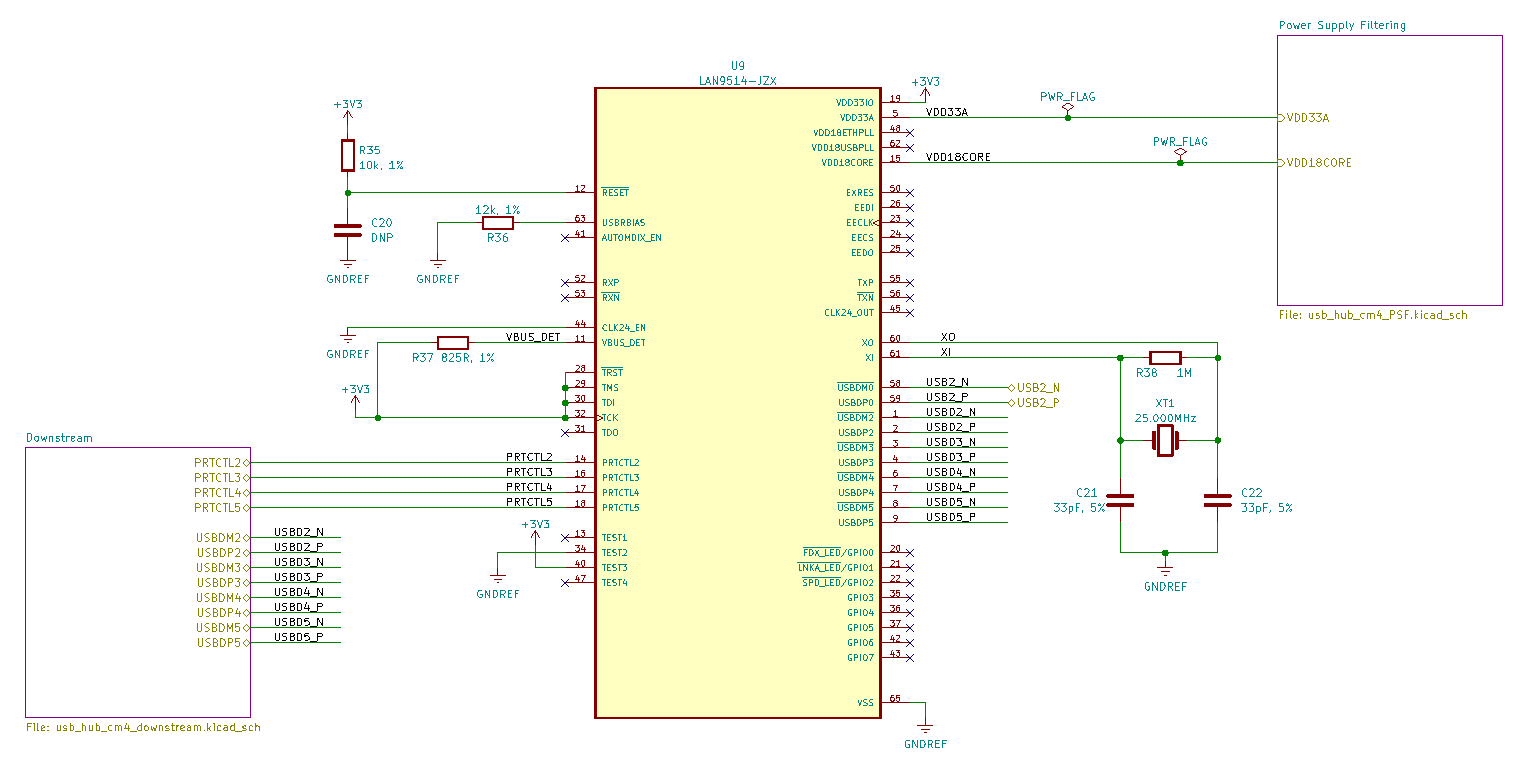
\includegraphics[width=1.0\textwidth]{Chapters/Figures/chapter3/USB_Hub_1.pdf}
	\caption{beRTK\textsuperscript{\textregistered} Base Station's USB Hub schematic diagram.}
	\label{fig:USB_Hub_1_circuit}
\end{figure}

% meter aqui circuito do USB_Hub_1
\begin{figure}[h]
	\centering
	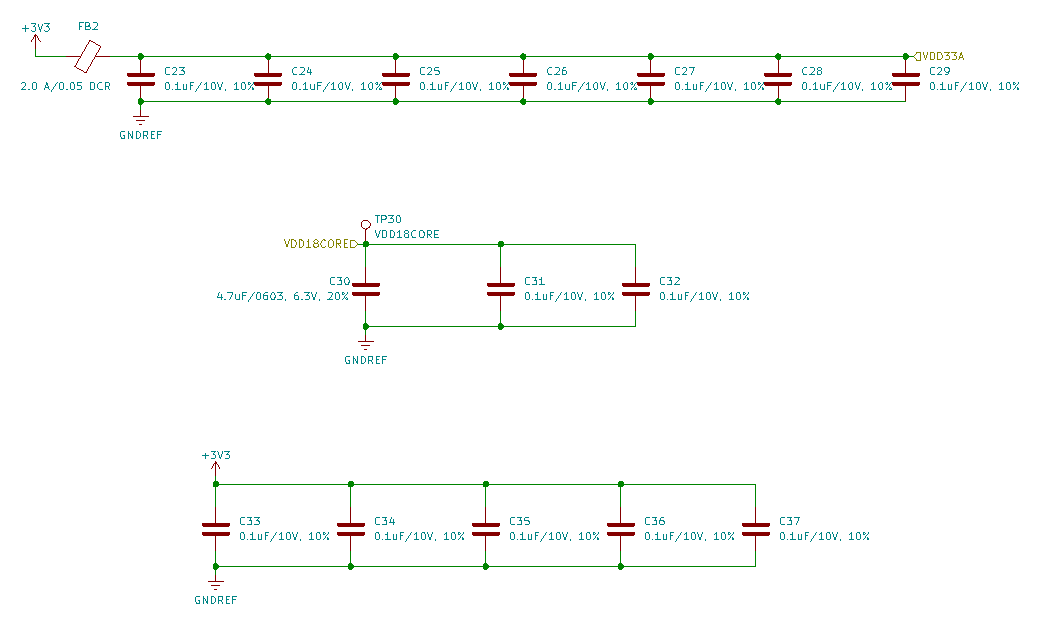
\includegraphics[width=1.0\textwidth]{Chapters/Figures/chapter3/USB_Hub_PwrSplyFiltering.pdf}
	\caption{beRTK\textsuperscript{\textregistered} Base Station's USB Hub's Power Supply Filtering schematic diagram.}
	\label{fig:USB_Hub_PwrSplyFiltering_circuit}
\end{figure}

% meter aqui circuito do USB_Hub_1
\begin{figure}[h]
	\centering
	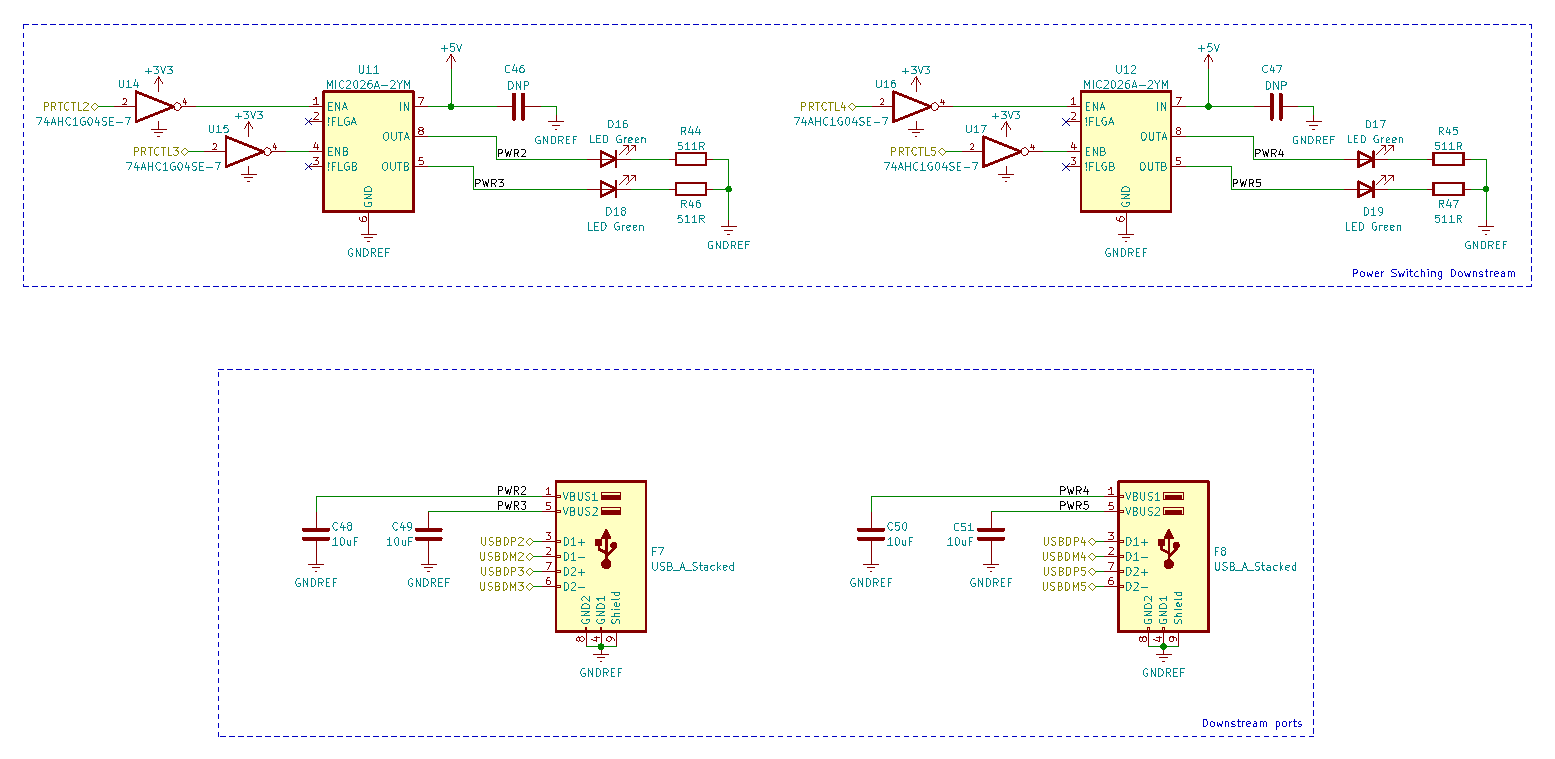
\includegraphics[width=1.0\textwidth]{Chapters/Figures/chapter3/USB_Hub_Downstream.pdf}
	\caption{beRTK\textsuperscript{\textregistered} Base Station's USB Hub's Downstream schematic diagram.}
	\label{fig:USB_Hub_Downstream_circuit}
\end{figure}

% REFERÊNCIA needed!!!!!!!!!!!!!!!!!!!!
%SSSSSSSSSSSSSSSSSSSSSSSSSSSSSSSSSSSSSSSSSSSSSSSSSSSSSSSSSSSSSSSSSSSSSSSSSSSS


\section{PCB Layout Design}\label{sec:33_PCBlayout}

-- $20 \mu$F ceramic capacitors were chosen for both the power inputs and power output of the LTC4012. 

-- As mentioned before, the top and bottom power FETs Q2 and Q9, along with inductor L1 are vital to the PWM control architecture. These components are part of the sub-circuit that starts from the +15VDC source of power and passes across FET Q1 (connected to pin INFET), sense resistor R3, 
This sub-circuit forms the ``power supply rail'', and upon layout design of the circuit from Figure~\ref{fig:LTC4012_circuit}, this section must bear a track width large enough to withstand large values of currents or any other phenomena that may occur (e.g. voltage/current spikes). The needed track width can be calculated through the following expression: